% version 1.0.0 (06/02/2019)
% version 1.0.1 (08/02/2019)
% version 1.1.0 (09/02/2019)
% version 1.1.1 (09/02/2019)
% version 1.1.2 (10/02/2019)
% version 1.1.3 (10/02/2019)
% version 1.1.4 (11/02/2019)
% version 2.0.0 (25/05/2019)
% version 3.0.0 (20/06/2019)

\documentclass{book}
\usepackage[paperwidth=150mm,%showframe,
paperheight=220mm,
textwidth=110mm,
inner=18mm,
includehead,
includefoot,
headsep=16pt,
top=15mm,
bottom=15mm,
marginparwidth=0mm,
marginparsep=0mm,
footskip=0mm]{geometry}
\usepackage{ragged2e}
% \usepackage{imagoLIBERTINUS}
\usepackage{bib-valbusaSC}
\addbibresource{ESTILO.bib}
\usepackage{CJKutf8}
\usepackage{fonttable}
\usepackage{marginnote}
\usepackage{IMglosario}
% \renewcommand*{\marginfont}{\color{blue}\sffamily\footnotesize\selectfont}
% \usepackage{xymtexpdf}
\usepackage{listings}
\renewcommand{\lstlistingname}{Listado de código}
\lstset{
language=Octave,
% frame=none,
breakatwhitespace=true,
breaklines=true,
numbers=left,
numbersep=14pt,
numberstyle=\tiny,
showstringspaces=false,
showtabs=false,
tabsize=2,
extendedchars=true,
keywordstyle=\color{blue},
commentstyle=\color{red},
% title=\lstname
}








% DISEÑO DE CAJA TIPOGRÁFICA
\newlength{\glyphwd}
\newcommand{\showglyph}[1]{%
 \begingroup
 \settowidth\glyphwd{#1}%
 \setlength{\fboxrule}{0.3pt}% hairline
 \setlength{\fboxsep}{-0.05pt}%
 \makebox[0pt][l]{\vrule height 0.05pt depth 0.05pt width \glyphwd}%
 \fbox{\textcolor{magenta}{#1}}%
 \endgroup
}

% % COMIENZO DEL EJERCICIO DE FUENTE
% \newlength\caph
% \newlength\desc
% \newlength\xlen
% \newlength\mlen
% \newcommand*{\prlen}[1]{%
%  % round to 1 digit:
%  \pgfmathparse{round(10*#1)/10.0}%
%  \pgfmathresult
% }

\newcommand{\Alphabet}{ABCDEFGHIJKLMNOPQRSTUVWXYZ}
\newcommand{\alphabet}{abcdefghijklmnopqrstuvwxyz}

\newcommand{\showfont}[1]{%
 \settoheight{\caph}{\Alphabet}%
 \settodepth{\desc}{\Alphabet\alphabet}%
 \setlength{\xlen}{1ex}%
 \setlength{\mlen}{1em}%
 \begin{tikzpicture}[
 every node/.style={inner sep=0pt},
 ]
 \path (0,0) node[anchor = south west] (A) {#1} ;
 \draw[black] (A.base west) -- (A.base east);
 \coordinate (Aex) at ($(A.base west)+(0,\xlen)$);
 \draw[black] (Aex) -- ($(A.base east)+(0,\xlen)$);
 \coordinate (Adesc) at ($(A.base west)-(0,\desc)$);
 \draw[black] (Adesc) -- ($(A.base east)-(0,\desc)$);
 \coordinate (Acaph) at ($(A.base west)+(0,\caph)$);
 \draw[black] (Acaph) -- ($(A.base east)+(0,\caph)$);
 \draw[magenta, thick] (Adesc) rectangle ++(\mlen, \mlen)
 coordinate (Amlen);
 %%
 \small\footnotesize\ttfamily
 \node [left=1em of A.base west, anchor=east, ] {l\'inea de base};
 \node [left=1em of Aex, anchor=east, ] {1ex=\prlen{\xlen} pt};
 \node [left=1em of Adesc, anchor=east, ] {descenso=\prlen{\desc} pt};
 \node [left=1em of Acaph, anchor=east, ] {caph=\prlen{\caph} pt};
 \node [above right =1em of Amlen, anchor=west, ] {1em=\prlen{\mlen} pt};
 \end{tikzpicture}%
}% FIN DEL EJERCICIO DE FUENTE

% % ACRóNIMO y GLOSARIO
\usepackage{glossaries}
% ACRóNIMO
% \newacronym{ONU}{\textcolor{magenta}{\textsc{onu}}}{Organización de las Naciones Unidas}
% \newacronym{si}{\textcolor{magenta}{\textsc{si}}}{Sistema Internacional de Unidades}
% \newacronym{AMS}{\textcolor{magenta}{\textsc{ams}}}{American Mathematical Society}
% \newacronym{CTAN}{\textcolor{magenta}{\textsc{ctan}}}{Comprehensive TeX Archive Network}

% GLOSARIO
% \newglossaryentry{aline}{name={Alineación},text={\textsc{alineación}},description={Refiere al posicionamiento del texto dentro de la caja o marco que lo contiene. La alineación puede ser a la izquierda, a la derecha, justificarse a ambos lados o centrarse}}
% \newglossaryentry{scriptum}{name={Post Scriptum},text={\textsc{post scriptum}},description={Es una locución latina que significa \enquote{{después de lo escrito}.​ Se emplea para agregar en los libros un texto posterior a su cierre o cuando este ya está dado por concluido, también es una alternativa a utilizar en las reediciones cuando no se quiere alterar el texto original}}}
% \newglossaryentry{postscript}{name={\textcolor{magenta}{PostScript.}},text={\textsc{postscript}},description={Es un lenguaje de programación utilizado para la descripción de páginas, se encuentra en muchas impresoras y también es muy común como formato para el transporte de archivos gráficos entre los distintos actores involucrados en un proceso de impresión (editorial, agencia de publicidad e imprenta)}}
% \newglossaryentry{tex}{name={\textcolor{magenta}{TeX.}},text={\textsc{tex}},description={Representado como \TeX, es un lenguaje de composición tipográfica escrito por Donald Ervin Knuth, muy popular en el entorno científico de las llamadas \enquote{{ciencias duras}. TeX se considera generalmente la mejor forma de editar fórmulas complejas, pero es a través de otros metalenguajes como \LaTeX, que su uso es más amigable en las tareas de edición}}
% \newglossaryentry{SI}{name={\textcolor{magenta}{Sistema internacional de unidades.}},text={si},description={Es el patrón de unidades adoptado por casi todos los países del mundo. Está constituido por siete unidades básicas y una gran cantidad de unidades derivadas y prefijos para denotar múltiplos y submúltiplos de las unidades. Los tres países que en su legislación no han reglamentado el SI son Birmania, Liberia y Estados Unidos}}
% \newglossaryentry{glifo}{name={\textcolor{magenta}{Glifo.}},text={\textsc{glifo}},description={En tipografía, un glifo (\emph{glyphs}) es la representación visual de un carácter, o de varios caracteres que son entendidos como uno solo. Mientras que un caracter es una unidad textual, un glifo es una unidad gráfica}}
% \newglossaryentry{ams}{name={\textcolor{magenta}{American Mathematical Society.}},text={\gls{AMS}},description={Es una sociedad estadounidense dedicada a los intereses de la investigación y patrocinio de las matemáticas, lo hace a través de varias publicaciones y conferencias así como con premios monetarios anuales que entrega a las investigaciones. La sociedad aboga por el uso del lenguaje de composición tipográfica \gls{tex}},user1={tex}}
% \newglossaryentry{ctan}{name={\textcolor{magenta}{Comprehensive TeX Archive Network.}},text={\gls{CTAN}},description={Es el sitio web de referencia para ubicar todo el material y \emph{software} relacionado con \gls{tex}},user1={tex}}

% ESTOS PAQUETES DEBEN IR AL FINAL DE LA CARGA
% \usepackage[citecolor=magenta,colorlinks=true,hyperfootnotes=false,pdftex]{hyperref}

\begin{document}
\frontmatter

% TAPA
\newpage
\thispagestyle{empty}
% {\textcolor{white}{.}}\\

\begin{center}

\includegraphics[width=.5\textwidth]{logo-estilo.pdf}

\vfill


\includegraphics[width=\textwidth]{logo-lion.pdf}
\end{center}

% RETIRACION DE TAPA
\newpage
\thispagestyle{empty}
{\textcolor{white}{.}}\\


%pagina 3
\newpage
\thispagestyle{empty}
\begin{center}
{\textcolor{white}{.}}
\vfill

\Large{Apunte urgente\\ del Manual de estilo de Ediciones Imago Mundi}\\
\vspace{12pt}
\large{versión 3.0.0}\\

\vfill
{\textcolor{white}{.}}
\end{center}

%pagina
\newpage
\thispagestyle{empty}
{\textcolor{white}{.}}\\

%pagina 5
\newpage
\thispagestyle{empty}
\begin{center}
\large{\textsc{alberto moyano}} \\

\vfill

\Large{Apunte urgente\\ del Manual de estilo de Ediciones Imago Mundi}\\
\vspace{12pt}
\large{versión 3.0.0}\\

\vfill


\includegraphics[width=20mm]{logo-imago-cmyk.pdf}
\end{center}

%pagina 6
\newpage
\thispagestyle{empty}
% {\textcolor{white}{.}}\\
\noindent Alberto Moyano\\
\noindent Apunte urgente del Manual de estilo de Ediciones Imago Mundi. Versión 3.0.0\\
% \noindent 87 p.; 15x22 cm.\\
\noindent ISBN 978-950-793-323-3\\
\noindent 1. Edición de Libros. I. Título \\
\noindent CDD 070.51092 \\
\noindent Fecha de catalogación: 06/01/2019\\
\noindent \textcopyright~2019, Alberto Moyano\\
\noindent \textcopyright~2019, Ediciones Imago Mundi\\
\noindent Tapa: el dibujo de tapa fue desarrollado por Duane Bibby, se puede obtener más información sobre el dibujo en la dirección \url{https://ctan.org/lion}.\\

\vfill

\begin{mdframed}[linewidth=.5pt,linecolor=black!30,roundcorner=3pt,backgroundcolor=yellow!15]
\noindent Este libro se distribuye a los lectores sin requerir pago alguno. Cualquier persona puede descargarlo, redistribuirlo y utilizarlo sin tener que pagar; aunque se mantienen intactos los derechos de autor y editorial y que, por tanto, no se permite modificar su contenido incluido el diseño de cubierta.
\end{mdframed}

\Author{Sumario}
\tableofcontents

\chapter{Advertencias para la lectura}
\Author{Alberto Alejandro Moyano}
{
\begin{compactitem}
\item Para facilitar la búsqueda de los terminos que se encuentran en el glosario de este libro. Los mismos son mostrados en \textsc{versalitas} a lo largo del texto.

\item Téngase en cuenta que este texto siempre será entendido como un parcial, ya que se encuentra con permanentes modificaciones. La forma de saber si está leyendo la última versión es comparando la que se indica en la web de la editorial con la que usted tiene.

Sobre el sistema de versiones he descartado el modelo utilizado en programación (x.y.z.p.t, incluyendo la instancia \emph{release candidate}), ya que después de leer varios textos sobre versionado para manuales, he concluido en que cada organización (o editorial) desarrolla su propio sistema, en Ediciones Imago Mundi usaremos x.y.z, donde:

\begin{compactdesc}
\item [\textbf{x:}] la primer cifra indica la versión mayor del documento. Cada cambio en este número indica modificaciones a nivel de estructura del libro. Cuando este número cambia, los valores siguientes se cuentan desde cero.
\item [\textbf{y:}] la segunda cifra indica la versión menor del documento, los cambios en este número significan que los mismos no son lo suficientemente importantes como para decir que ya no es el mismo documento.
\item [\textbf{z:}] la tercera cifra sugiere cambios menores, por ejemplo realizar correcciones a errores ortográficos.
\end{compactdesc}
\end{compactitem}

% \chapter{Advertencia}
% \Author{Alberto Moyano}
%
% \noindent \textbf{EXPLICAR LOS HIPERVINCULOS}
%
%
%
% Al margen de lo planteado en el párrafo anterior, si usted es autor puede obviar las advertencias indicadas a continuación, ya que las mismas están dirigidas a tipógrafos y editores, o en su defecto a estudiantes de estas disciplinas.
%
% \begin{compactdesc}
% \item [\textcolor{magenta}{\textbf{\textbf{Si usted es tipógrafo o editor:}}}] el principal cambio está en que he cambiado el \emph{driver} de salida, dejo atrás pdfLaTeX para pasar a usar LuaLaTeX. Las diferencias entre estos dos \emph{drivers}, son radicales en muchas cuestiones pero fundamentalmente en el tratamiento de las tipografías, básicamente LuaLaTeX maneja las tipografías OpenType de manera directa, sin pasar por (ni depender) el sistema operativo que se utilice (MacOS, Windows o Linux), y de esta manera accede a todas las capacidades de la misma.
% \end{compactdesc}

\chapter{Agradecimiento}

\noindent Donald Ervin Knuth\index[apellidos]{Knuth, Donald Ervin} es una persona a quien no conozco personalmente, pero utilizo su desarrollo informático como herramienta de trabajo en el día a día, también están los aportes de otras personas (y muchos de ellos son extremadamente valiosos), pero todo sigue girando en torno al núcleo principal que él desarrolló, por eso siento necesario hacer explícito este agradecimiento en particular.

Knuth es profesor de matemáticas y computación en la Universidad de Stanford, en la actualidad es catedrático emérito. Es considerado uno de los padres fundadores de la informática moderna, e incluso de Internet. Su libro \emph{The Art of Computer Programming} (\cite*{Knuth2011}) es una de las más respetadas referencias en el campo de las ciencias de la computación.

En 1977 comenzó a desarrollar el lenguaje\index[conceptos]{lenguaje} \gls{tex} en su año sabático, con el apoyo de la Universidad de Stanford y la editorial Addison Wesley; han pasado más de 40 años desde que Knuth comenzó su desarrollo y al día de hoy todavía sigue siendo el más refinado y perfecto sistema de composición tipográfica digital que exista: para explicitar lo obvio, \gls{tex} no es un programa de armado de páginas, es un \emph{lenguaje de edición y composición tipográfica}.\index[conceptos]{lenguaje!de composición tipográfica} Y no ha dejado de evolucionar desde que se hizo público, gracias a su licencia de \emph{software} libre. Tiene una amplia y variada comunidad de colaboradores detrás, formada principalmente por universidades e instituciones \ \ldash{como la \gls{AMS}}\rdash \ y muchos particulares teóricos de la edición y la tipografía, \gls{tex} no es un simple \emph{software}: es una disciplina en sí, que conlleva la obligación en el día a día \ \ldash{a quien lo utiliza}\rdash \ de sostener un permanente aprendizaje. En su uso no hay espacio para la intuición \ \ldash{donde radica la mayor parte de la crítica que recibe}\rdash \ pero de eso se trata, de comprender y saber; por qué y para qué.

\gls{tex} se encuentra realmente a años luz de los programas estándares más utilizados en la industria editorial para la composición y edición de libros (\emph{e.g.} InDesign, XPress, Scribus, etcétera); pero es incorrecto \ \ldash{rozando lo injusto}\rdash \ hacer comparaciones, ya que \gls{tex} como lenguaje,\index[conceptos]{lenguaje} es un \emph{software} que provee las mismas libertades y posibilidades de manipulación de los contenidos que se tienen cuando se trabaja de manera manual, esto significa que el límite para los resultados que se pueden obtener están directamente ligados al conocimiento que se tengan del lenguaje mismo, a diferencia de los programas estándares de la industria, en donde los límites de lo que se puede o no hacer están ligados al grado de evolución que el \emph{software} posea.

También es posible observar que en la edición de libros \ \ldash{al menos hasta el día de hoy}\rdash \ el \emph{software} estándar del mercado está enfocado en la diagramación y el armado, utilizando de manera obligatoria la acción visual. En \gls{tex} se piensa y se trabaja desde otra perspectiva \ \ldash{el foco se encuentra en la edición}\rdash \ por eso cuando tratamos de manipular textos para la composición de páginas o incluso la automatización de diversos procesos que incluyan páginas \ \ldash{y un listado bastante largo de posibilidades}\rdash \ los programas convencionales del mercado no pueden ser entendidos como competidores de \gls{tex}. Aunque es necesario aclarar que varias editoriales como Adison Wesley, Elsevier, Teub­ner, Ver­lag y Mentis,\footnote{Estas son solo algunas, que incluso han desarrollado paquetes ajustados a sus estilos para ser utilizados por los autores, en otras palabras, las editoriales reciben los artículos \enquote{{prearmados}.} ya han adoptado el lenguaje \gls{tex}.

% Solo es necesario recorrer el \gls{ctan} para observar que \gls{tex} no es ideal unicamente para producir fórmulas matemáticas. Al momento de escribir este texto existen \num{5632} paquetes de colaboradores, con \num{2574} personas contribuyendo a ello. La mayoría de los paquetes son de uso gratuito y se pueden descargar y utilizar en el momento.

\gls{tex} como lenguaje\index[conceptos]{lenguaje} es extremadamente dúctil y potente, se pueden producir todo tipo de libros, desde los más simples hasta los muy complejos y siempre con una esmerada atención por el respeto a las distintas tradiciones editoriales y tipográficas.

\chapter{Prefacio}

\noindent A mediados de 2018 me propuse escribir un manual de estilo para la editorial; hice un trazado de lineamientos, arme la primera matriz de contenido y sume algunos colaboradores en temas específicos; cuando me quise dar cuenta tenía entre manos un proyecto muy ambicioso \ \ldash{en tiempo y cantidad de páginas}\rdash \ que está más cerca de ser un manual de edición antes que el manual de estilo de la editorial, frente a esto, consideré necesario tener esta salida resumida, que di en llamar \emph{Apunte urgente del Manual de estilo de Ediciones Imago Mundi}, eso es lo que el lector va a encontrar en estas páginas.

\epigraph{\enquote{{Estándar: (adjetivo) que sirve como tipo, modelo, norma, patrón o referencia}.}{\textcite{RAE2010}}

La definición de la RAE refleja qué es lo que Ediciones Imago Mundi busca obtener, lo que no dice es que muchas veces \ \ldash{y esta es una}\rdash \ un estándar también puede ser el resultado de muchos años de trabajo. Han pasado más de 15 años de constante intercambio de conocimiento con espacios que funcionan como puntos de retroalimentación. En este fluir es importante resaltar que el liderazgo lo han llevado y continua siendo de las universidades, así como tampoco debe sorprender que la composición tipográfica sea el eje de partida para todos los involucrados.

Tipógrafos, gráficos, historiadores, editores, matemáticos, etcétera, que trabajan en diferentes universidades del globo, así como también en empresas privadas o que de manera particular, aportan cotidianamente soluciones al foro de \gls{tex},\footnote{Con más de \num{170000} preguntas al día de hoy y con más de \num{3700} usuarios activos, es el lugar de consulta por excelencia, junto a la calidad de muchas de sus respuestas (\url{https://tex.stackexchange.com}).} la lista de CervanTeX,\footnote{CervanTeX es el grupo de usuarios hispanohablantes de TeX, y forma parte de los grupos locales asociados al TUG (\url{http://www.cervantex.es}).} el \gls{ctan}\footnote{El \gls{CTAN} proporciona acceso a los diferentes directorios y archivos ubicados en el repositorio \url{https://ctan.org}.} y el TUG.\footnote{El TeX Users Group (TUG) fue fundado en 1980 para proporcionar una organización a aquellas personas interesadas en el uso del sistema de composición \gls{tex} inventado por Donald Ervin Knuth\index[apellidos]{Knuth, Donald Ervin} (véase \url{http://tug.org}).}

\textcite[125]{Furtado2014} plantea que en una primera aproximación, las editoriales se distinguen entre ellas por la predominancia que tienen sus actividades primarias en la transformación físico-técnicas del contenido; desde el punto de vista de la editorial, esto implica que el componente de producción (y la calidad del contenido trabajando sinergicamente) gozan de mucho valor.

Este libro está dirigido principalmente a autores, y aunque son muchos los puntos que quedaron sin incluir \ \ldash{que son parte del \emph{Manual}}\rdash \ pueden sacar provecho de él todas aquellas personas que de alguna manera estén interesadas en la edición, sean estudiantes, docentes o público en general, ya que encontrarán acá un punto de referencia.

Todo el contenido lleva la concepción de un libro \enquote{{promedio} en estructura, esto es, se van a encontrar todas las áreas que a su vez están explicadas en el interior del mismo; los listados al final son cortos, ya que solo llevan la idea de ser ilustrativos.

\mainmatter

\chapter{Presentación de los recursos}

\section{Introducción}

En Ediciones Imago Mundi abandonamos el concepto de \emph{documento}, que fue el más comúnmente utilizado para la descripción de libros, revistas y similares, y hemos empezado a utilizar el término \emph{recurso}, que es mucho más abarcativo, ya que incluye a los medios electrónicos y audiovisuales, este cambio obedece a que hoy son muy variadas las fuentes disponibles para la investigación científica.

\section{Material previamente publicado}

Si el libro que ingresa a producción ya ha sido previamente publicado por otra editorial, se deberá entregar a Ediciones Imago Mundi una copia impresa de dicha edición.

\section{Los originales}

El trabajo original se debe entregar en soporte digital, los formatos permitidos son los provistos por Microsoft Office y Libre Office. Las páginas se configurarán en formato A4. Para el cuerpo del texto se utilizará tipografía Times New Roman cuerpo 12 con interlineado 1,5. Los archivos se consignarán según se muestra en el listado a continuación, solo se deben entregar los que correspondan:

\begin{compactenum}
\item un archivo único con el índice y los datos del autor o editor;
\item un archivo único con todos los capítulos que componen el libro, siguiendo el orden de aparición;
\item un archivo único con la bibliografia completa de todo el libro;
\item un archivo único con el listado de acrónimos de todo el libro;
\item un archivo único con el listado de glosario de todo el libro;
\item un archivo único con el listado de palabras claves de todo el libro;
\item tantos archivos en formato de imagen como sean necesarios, uno por cada imagen. Asimismo las fotografías deberán ser colocadas dentro del archivo único que contiene todos los capítulos, solo a modo de ejemplo para su ubicación orientativa;
\item tantos archivos de planillas de cálculo como sean necesarios, uno por cada figura, estos son necesarios debido a que las figuras provistas no son utilizadas, sino que son construidas utilizando los datos. Si las planillas poseen archivos vinculados, estos también deberán ser provistos. Las figuras deberán ser colocadas dentro del archivo único que contiene todos los capítulos, solo a modo de ejemplo para su ubicación.
\end{compactenum}

\section{Me leo y no me gusto}

Ha pasado en algunas oportunidades que los autores al poco tiempo de enviado los archivos para el proceso de edición, envíen una nueva versión del texto; estos archivos no son recibidos ya que ocasionan mayores costos, esto se debe a que los archivos una vez entregados a la editorial pasan inmediatamente a control y corrección.

Por los motivos antes expuestos se hace necesario recalcar a los autores de la importancia de entender que la versión de archivo que envían para producción, es considerada como la definitiva.

\section{Tengo una parte, podemos adelantar}

Si el libro tiene fecha certera de salida, por lo general obedeciendo a compromisos pre pactados, pero los textos finales no están en la fecha \ \ldash{también pre pactada}\rdash \ necesaria, no será posible cumplir con el compromiso de salida.

Lamentablemente, no podemos trabajar con textos a medias, para el proceso de edición se necesitan todos los elementos en su versión definitiva.

\section{Diferencia entre imagen y figura}

\begin{compactdesc}
\item [\textcolor{magenta}{\textbf{Qué entendemos por imagen:}}] es la representación gráfica de algo real, que se obtiene a través de  algún proceso químico o electrónico;
\item [\textcolor{magenta}{\textbf{Qué entendemos por figura:}}] es la representación gráfica de un dibujo, que se obtiene a través de cálculos matemáticos o químicos y que se utiliza para expresar algo.
\end{compactdesc}

\subsection{Imágenes}

Las imágenes serán provistas en cualquiera de los siguientes formatos: {\ttfamily .png}, {\ttfamily .jpg} o cualquiera de ellos que se encuentre dentro de un {\ttfamily .pdf}, la resolución no debe ser inferior a 200 dpi en escala 1:1 del tamaño de salida.

\begin{imagen}
\includegraphics[width=\textwidth]{barrendero.jpg}
\caption{Fuente: Archivo General de la Nación.}
\end{imagen}

\subsection{Figuras}

Las figuras son desarrolladas por la editorial utilizando los datos de las planillas de cálculo o archivos de texto plano entregadas en alguno de los lenguajes\index[conceptos]{lenguaje} más comunes a este fin: Libre Office Calc, Microsoft Excel, R, Octave y MathLab.

\begin{figure}[!ht]\cuadrosTTT
\begin{mdframed}[linewidth=.5pt,linecolor=black!30,roundcorner=3pt]
\centering
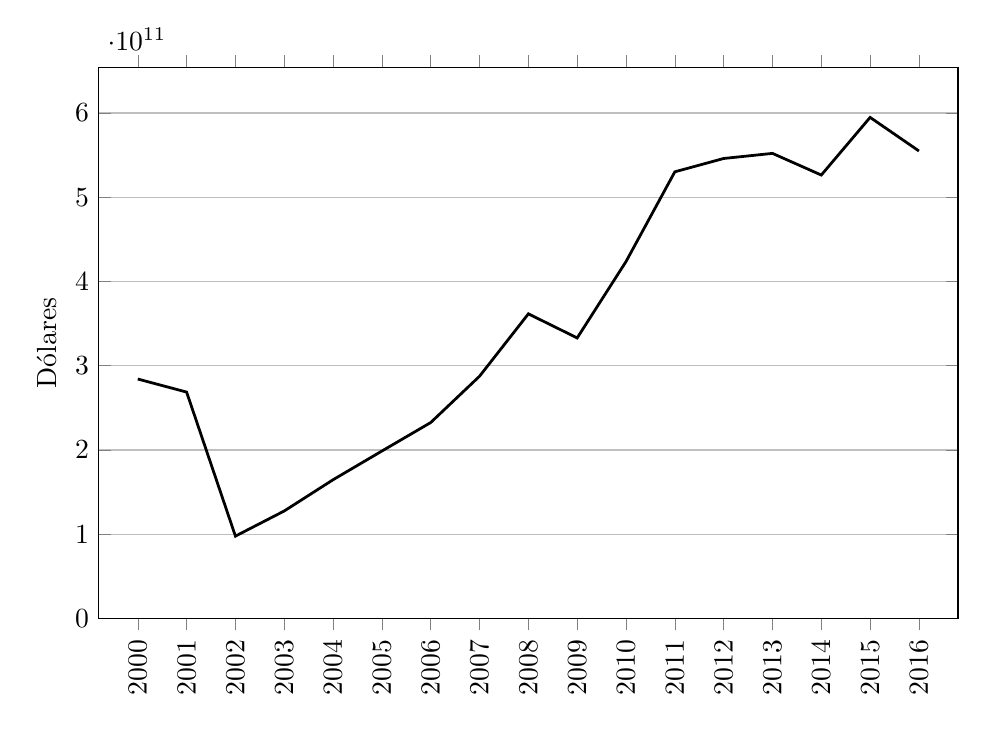
\begin{tikzpicture}
\begin{axis}[width=.9\textwidth,
	      height=7cm,
	      scale only axis,
	      ybar,
	      ymajorgrids = true,
	      ymin=1000000,
	      ylabel={Dólares},
% 	      ymax=200,
	      enlarge x limits={value=.05,auto},
	      symbolic x coords={2000,2001,2002,2003,2004,2005,2006,2007,2008,2009,2010,2011,2012,2013,2014,2015,2016},
	      xtick=data,
	      x tick label style={/pgf/number format/1000 sep=,},
	      xticklabel style={rotate=90,anchor=east}]
\addplot[line width=1pt, mark=none, black, sharp plot] coordinates %
{(2000,284203750000)
 (2001,268696750000)
 (2002,97724004251.8602)
 (2003,127586973492.177)
 (2004,164657930452.787)
 (2005,198737095012.282)
 (2006,232557260817.308)
 (2007,287530508430.568)
 (2008,361558037110.419)
 (2009,332976484577.619)
 (2010,423627422092.49)
 (2011,530163281574.658)
 (2012,545982375701.128)
 (2013,552025140252.246)
 (2014,526319673731.638)
 (2015,594749285413.212)
 (2016,554860945013.62)};
\end{axis}
\end{tikzpicture}
\caption{Figura desarrollada tomando datos de una planilla de cálculo.}
\end{mdframed}
\end{figure}

\section{Trabajando con itemizados \label{itemizados}}
% \marginnote{\textcolor{blue}{\footnotesize\sffamily \textbf{v. 1.1.0}}}

Ediciones Imago Mundi sugiere descartar hacer itemizados dentro de la redacción, como propuesta ofrece dos modelos con hasta tres niveles de anidamiento,\footnote{El anidamiento es la práctica de incorporar llamadas unas dentro de otras, mediante la inclusión de separadores.} cada uno obedece a diferentes necesidades de redacción. El primer modelo tiene el concepto enumerativo, las líneas terminan con punto y coma, ya que se considera que todo el bloque debe ser entendido como uno. El segundo tiene el concepto de líneas autónomas entre sí, por ese motivo terminan en punto.

\begin{mdframed}[linewidth=.5pt,linecolor=black!30,roundcorner=3pt]
\begin{compactenum}
\item primer item (primer nivel);
	\begin{compactenum}
	\item primer item (segundo nivel);
		\begin{compactenum}
		\item primer item (tercer nivel);
		\item segundo item (tercer nivel);
		\end{compactenum}
	\item segundo item (segundo nivel);
	\end{compactenum}
\item segundo item (primer nivel).
\end{compactenum}
\end{mdframed}

\begin{mdframed}[linewidth=.5pt,linecolor=black!30,roundcorner=3pt]
\begin{compactitem}
\item Primer item (primer nivel).
	\begin{compactitem}
	\item Primer item (segundo nivel).
		\begin{compactitem}
		\item Primer item (tercer nivel).
		\item Segundo item (tercer nivel).
		\end{compactitem}
	\item Segundo item (segundo nivel).
	\end{compactitem}
\item Segundo item (primer nivel).
\end{compactitem}
\end{mdframed}

\section{Algunos consejos}

A continuación se verá un listado general de pautas para la escritura de los originales, las mismas intentan ser un conjunto de indicaciones generales que los autores pueden seguir para unificar un criterio de escritura estandarizado. Este listado debe ser considerado parcial, ya que este manual se encuentra en permanente actualización.

\subsection{Control de cambios}

Los archivos deben ser entregados con el control de cambios desactivado, para que no exista el riesgo de que queden modificaciones sin volcar de manera definitiva.

\subsection{Sin abreviaturas}

Los nombres propios de los diferentes intervinientes dentro del libro y en la bibliografía, no deben ser abreviados. Para las fuentes orales, en los casos en los que se necesita salvaguardar el nombre del entrevistado, se puede considerar el uso de un apodo.

\subsection{Diacríticos y otros caracteres}

A menos que por razones técnicas o de desconocimiento sea imposible, es obligatorio respetar la escritura con diacríticos y otros caracteres alfabéticos, estos son algunos ejemplos.

\begin{mdframed}[linewidth=.5pt,linecolor=black!30,roundcorner=3pt,backgroundcolor=yellow!15]
\large\selectfont
\centering
Fran\textcolor{magenta}{ç}ois, Ric\textcolor{magenta}{\oe}{}ur, Varj\textcolor{magenta}{ã}o, \textcolor{magenta}{Ž}i\textcolor{magenta}{ž}ek, Gr\textcolor{magenta}{üß}edich, \begin{CJK}{UTF8}{mj}\textcolor{magenta}{문정현}\end{CJK}
\end{mdframed}

\subsection{Comillas}

\subsubsection{Tipos de comillas}

En el cuadro~\ref{comillas} se puede observar el diseño del \gls{glifo} para los idiomas más comúnmente utilizados en Ediciones Imago Mundi, para el español utilizamos primero las comillas dobles angulares y en segundo nivel las comillas dobles inglesas.

También es posible observar en todos los idiomas mostrados (menos el francés) que todas las comillas de apertura se escriben pegadas al primer \gls{glifo} contiguo y todas las de cierre pegadas al último, sin dejar ningún espacio; para el francés la distancia es de 1/4 em. Lo adecuado es además, que el punto, la coma, el punto y coma y los dos puntos se escriban fuera de las comillas de cierre.

\begin{table}[!h]
\begin{mdframed}[linewidth=.5pt,linecolor=black!30,roundcorner=3pt,backgroundcolor=yellow!15]
\centering
\begin{tabular}{ll}
\toprule
Español & \large{\enquote{\textcolor{magenta}{Hola} \enquote{\textcolor{magenta}{pequeño mundo}}}\textcolor{magenta}{.}} \\
\midrule
Inglés & \large{\selectlanguage{english}\enquote{\textcolor{magenta}{Hello} \enquote{\textcolor{magenta}{little world}}}\textcolor{magenta}{.}}\\
\midrule
Portugués & \large{\selectlanguage{portuguese}\enquote{\textcolor{magenta}{Olá} \enquote{\textcolor{magenta}{mundo pequeno}}}\textcolor{magenta}{.}}\\
\midrule
Francés & \large{\selectlanguage{french}\enquote{\textcolor{magenta}{Bonjour} \enquote{\textcolor{magenta}{petit monde}}}\textcolor{magenta}{.}}\\
\midrule
Alemán & \large{\selectlanguage{german}\enquote{\textcolor{magenta}{Hallo} \enquote{\textcolor{magenta}{kleine Welt}}}\textcolor{magenta}{.}}\\
\bottomrule
\end{tabular}
\caption{}\label{comillas}
\end{mdframed}
\end{table}

\selectlanguage{spanish}

\subsubsection{Comillas de seguimiento}

Las comillas de seguimiento se utilizan cuando en una cita textual se reproduce el texto de otro autor y esta se conforma de varios párrafos, mientras que el primer párrafo comienza con el signo de apertura de comillas («), en los párrafos siguientes se implementa al inicio y sin espacio entre el signo y el caracter contiguo, la comilla de seguimiento (o continuación) el signo ortográfico utilizado es la comilla angular de cierre (»).

Siempre que se inicia una cita de un solo párrafo es necesario cerrarla con el signo de cierre de comillas (»), pero no se cierra cada uno de los párrafos cuando la cita está conformada por varios, y solo se cierra el último párrafo de la cita. Ediciones Imago Mundi no coloca sangría a los párrafos.

\begin{mdframed}[linewidth=.5pt,linecolor=black!30,roundcorner=3pt,backgroundcolor=yellow!15]
\begin{myquote}
\enquote{{(\dots) desde fines del siglo~XIX y hasta hace pocos años, el valle Calchaquí en general y el santamariano en particular fueron construidos como zonas en las que el problema del indio se dio por terminado con las desnaturalizaciones.

En el mejor de los casos, el valle fue pensado como espacio mestizo, en el que la impronta indígena se evaneció definitivamente hacia fines del siglo~XVII}.
\end{myquote}
\end{mdframed}

\subsection{Volumen \emph{versus} tomo}

En el texto solo se deben consignar las divisiones que corresponden a las partes y los tomos, en caso de corresponder; para mayor detalle sobre esta división, véase la sección~\ref{tomovolumen}, en la pág.~\pageref{tomovolumen}.

\subsection{Citas}

Recomendamos como regla que las citas con menos de treinta palabras permanezcan dentro del texto entre comillas dobles angulares: \textcolor{magenta}{\enquote{{Según Zamora, la realidad fue más sencilla: los candidatos propuestos para la JRG dentro de la DC habían sido Morales Erlich y Fidel Chávez Mena}} \parencite[154]{MenjivarOchoa2006}. Esta regla no se cumple cuando las citas son diálogos.

Las citas con más de treinta palabras, deben ser colocadas en un nuevo párrafo, Ediciones Imago Mundi utiliza en su diseño sangría sobre el margen izquierdo de 14pt. Se puede observar el siguiente ejemplo:

\begin{mdframed}[linewidth=.5pt,linecolor=black!30,roundcorner=3pt,backgroundcolor=yellow!15]
\begin{myquote}
\enquote{{Según Zamora, la realidad fue más sencilla: los candidatos propuestos para la JRG dentro de la DC habían sido Morales Erlich y Fidel Chávez Mena. Chávez, el hombre de Duarte (\dots), había trabajado en arreglos políticos que serían rechazados por la DC, como el armado del Foro Nacional de Carlos Humberto Romero y negociaciones paralelas con los militares \ \ldash{de las que hablan Gutiérrez y Majano}\rdash \ y con funcionarios de la embajada estadounidense. Los propios progresistas se lo plantearon a Dada: era él o Chávez, y la decisión fue obvia. Dada, durante la primera etapa de la JRG, aunque con posiciones definidas, había dado muestras de tolerancia dentro del sector progresista; Rubén Zamora y Jorge Villacorta, más confrontativos, no serían bien recibidos por los militares, y Mario Zamora aún ocupaba la Procuradoría General de la República} \parencite[154]{MenjivarOchoa2006}.
\end{myquote}
\end{mdframed}

\subsection{Cuadros}

\subsubsection{Cuadro en vez de tabla}

Si bien es una condición que debe ser revisada en cada edición, para la mayoría de los textos es correcto el uso de la expresión \enquote{{cuadro}, y no el de \enquote{{tabla}, que nos dice la \textcite{RAE2010}.

\begin{compactitem}
\item \textbf{Tabla} (11 f): lista o catálogo de cosas puestas por orden sucesivo o relacionadas entre sí. \emph{La tabla periódica de los elementos químicos}.
\item \textbf{Tabla} (12 f): cuadro o catálogo de números de especie determinada, dispuestos en forma adecuada para facilitar los cálculos. \emph{Tabla de multiplicar, de logaritmos, astronómica}.
\item \textbf{Cuadro} (9 m): conjunto de nombres, cifras u otros datos presentados gráficamente, de manera que se advierta la relación existente entre ellos.
\end{compactitem}

Y la explicación de Javier Bezos\index[apellidos]{Bezos, Javier} resulta mucho más clara:

\begin{myquote}
\enquote{{A pesar de su similitud, el inglés \emph{table} no es el español tabla (se habla de falsos amigos, es decir, palabras similares en dos lenguas pero con significados distintos)}.
\end{myquote}

\subsubsection{El signo negativo}

Cuando hablamos de valores matemáticos, la palabra signo se refiere a su propiedad. Todos los números distintos de cero son positivos o negativos, y tienen por tanto un signo que los identifica, para los valores mayores a cero, se omite escribir el signo positivo, pero para los valores menores de cero se adiciona por delante el signo negativo.

\begin{table}[!ht]\cuadrosTTT
\begin{mdframed}[linewidth=.5pt,linecolor=black!30,roundcorner=3pt,backgroundcolor=yellow!15]
\centering
\begin{tabular}{l | S[table-format=5.0] |
		  S[table-format=5.0] |
		  S[table-format=5.0] |
		  S[table-format=2.1] |
		  S[table-format=2.1] |
		  S[table-format=2.1]}
\toprule
 & \multicolumn{3}{c |}{\textbf{Datos absolutos}} & \multicolumn{3}{c}{\textbf{Variaciones rel. (\%)}} \\
\cmidrule{2-7}
\textbf{Provincias} & {\textbf{1988}} & {\textbf{2002}} & {\textbf{2008}} & {\textbf{1988/02}} & {\textbf{2002/08}} & {\textbf{1988/08}} \\
\midrule
Catamarca & 9538 & 9138 & 9012 & -4.2 & -1.4 & -5.5 \\
\midrule
Jujuy & 8526 & 8983 & 8733 & 5.4 & -2.8 & 2.4 \\
\midrule
Salta & 9229 & 10297 & 10317 & 11.6 & 0.2 & 11.8 \\
% \midrule
% Sgo. del Estero & 21122 & 20949 & 15899 & -0.8 & -24.1 & -24.7 \\
\midrule
Tucumán & 16571 & 9890 & 7669 & -40.3 & -22.5 & -53.7 \\
\midrule
NOA & 64986 & 59257 & 51630 & -8.8 & -12.9 & -20.6 \\
\bottomrule
\end{tabular}
\caption{Evolución de la cantidad de EAPs. Región NOA (1988, 2002, 2008).}
\end{mdframed}
\end{table}

\subsection{Bastardillas, negritas y subrayados}

El uso de las bastardillas se reserva para las palabras en idioma diferente al principal del texto, están exceptuados de esta regla los nombres propios y las referencias bibliográficas.

Para los casos en los que el autor considere la necesidad de aplicar énfasis a algunas palabras o pequeñas expresiones, se debe dar privilegio al uso de las comillas.

Las negritas (\emph{bold}) y el subrayado, están descartados para ser utilizados en el cuerpo principal del texto, y solo serán usados de manera muy excepcional.

\subsection{La raya}

Dentro de un buen trabajo de edición es aconsejable controlar que estos cuatro signos (raya corta, raya media, raya larga y signo menos) no se confundan, ya que son muy similares.\footnote{Incluso es muy común encontrar que a todos se los llame guiones.}

\begin{table}[!h]
\begin{mdframed}[linewidth=.5pt,linecolor=black!30,roundcorner=3pt,backgroundcolor=yellow!15]
\centering
\begin{tabular}{m{6cm} | l}
\toprule
Raya corta para corte de palabra estándar de la tipografía & \large{-\textcolor{magenta}{Hola Mundo}-} \\
\midrule
Raya media estándar de la tipografía & \large{--\textcolor{magenta}{Hola Mundo}--}\\
\midrule
Raya larga estándar de la tipografía & \large{---\textcolor{magenta}{Hola Mundo}---}\\
% \midrule
% Raya media diseñada por Ediciones Imago Mundi, obsérvese que es un poco más corta y tiene modificada la separación con su caracter contiguo & \large{\ldash{\textcolor{magenta}{Hola Mundo}}\rdash}\\
\midrule
Signo menos, este es el utilizado por \gls{tex} para indicar valores negativos & \large{$-$\textcolor{magenta}{\tt{\num{8012}}}}\\
\bottomrule
\end{tabular}
\end{mdframed}
\end{table}

\subsection{Tilde en las mayúsculas}

Las mayúsculas siempre deben llevar tilde en los casos en los que corresponda. Esta regla no se cumple cuando se trata de un acrónimo. Véanse los ejemplos:

\begin{mdframed}[linewidth=.5pt,linecolor=black!30,roundcorner=3pt,backgroundcolor=yellow!15]
\begin{compactitem}
\item África
\item AMÉRICA
\item IDH (Índice de Desarrollo Humano)
\end{compactitem}
\end{mdframed}

\subsection{Disciplinas científicas}

Los sustantivos y adjetivos de los nombres de disciplinas científicas van siempre en minúscula, no así cuando refiere a la asignatura y/o materia. Véanse los ejemplos:

\begin{mdframed}[linewidth=.5pt,linecolor=black!30,roundcorner=3pt,backgroundcolor=yellow!15]
\begin{compactitem}
\item estudiar matemáticas es apasionante
\item conozco a esa persona, es profesora de Geografía
\end{compactitem}
\end{mdframed}

\subsection{Hipervínculos}

Los textos no deben contener hipervínculos activos de ningún tipo, siga estas instrucciones para desactivarlos en Microsoft Word:

\begin{mdframed}[linewidth=.5pt,linecolor=black!30,roundcorner=3pt,backgroundcolor=yellow!15]
\begin{myquote}
Para quitar todos los hipervínculos de un documento, presione CTRL+A para seleccionar el texto en todo el documento, a continuación, presione CTRL + MAYÚS + F9.
\end{myquote}
\end{mdframed}

\noindent y estas para Libre Office:

\begin{mdframed}[linewidth=.5pt,linecolor=black!30,roundcorner=3pt,backgroundcolor=yellow!15]
\begin{myquote}
Abra primero un documento de texto. Vaya a \emph{Herramientas} --> \emph{Corrección automática} --> \emph{Opciones de corrección automática}.

En el cuadro de diálogo \emph{Corrección automática}, seleccione la pestaña \emph{Opciones}. Debe quitar la marca de la casilla \emph{Reconocer URL}, a partir de ahora ninguna palabra se reemplazará automáticamente por un hipervínculo.
\end{myquote}
\end{mdframed}

\subsection{Fechas}

No corresponde utilizar el apóstrofo para representar los años junto a sus dos últimas cifras: '98 por 1998. Si la abreviatura fuese necesaria o es una elección en la escritura, debe hacerse sin el apóstrofo.

\begin{mdframed}[linewidth=.5pt,linecolor=black!30,roundcorner=3pt,backgroundcolor=yellow!15]
\begin{compactitem}
\item verano del 68
\end{compactitem}
\end{mdframed}

\subsection{Letras}

Las décadas se escriben con letra y no con cifras. Es igualmente incorrecto escribirlas en plural.

\begin{mdframed}[linewidth=.5pt,linecolor=black!30,roundcorner=3pt,backgroundcolor=yellow!15]
\begin{compactitem}
\item los años setenta significaron\dots
\end{compactitem}
\end{mdframed}

\subsection{Horas}

Las marcas horarias se escribirán con números y en el formato de 24 horas, se utilizan los dos puntos para separar los elementos que integran la expresión horaria (18:47).

De acuerdo con el estándar internacional, deben emplearse dos dígitos para cada elemento (03:07, 22:00). En las horas en punto pueden omitirse los ceros si se utiliza el símbolo h (22 h).

\subsection{Estado o estado}

Se escribe \enquote{{Estado}, con inicial mayúscula cuando se alude a una forma de organización política, poder soberano e independiente, que integra la población de un territorio o al conjunto de los órganos de gobierno de un país soberano, esto vale tanto para el singular como para el plural. Entonces, se escriben con mayúscula:

\begin{mdframed}[linewidth=.5pt,linecolor=black!30,roundcorner=3pt,backgroundcolor=yellow!15]
\begin{compactitem}
\item Estado argentino;
\item Estado federal;
\item golpe de Estado;
\item razón de Estado;
\item seguridad del Estado;
\item secreto de Estado;
\item Estado de derecho;
\item Consejo de Estado;
\item jefe de Estado.
\end{compactitem}
\end{mdframed}

También se emplea la mayúscula en las expresiones que hacen referencia a las fuerzas armadas:

\begin{mdframed}[linewidth=.5pt,linecolor=black!30,roundcorner=3pt,backgroundcolor=yellow!15]
\begin{compactitem}
\item Estado Mayor;
\item Estado Mayor Central;
\item Estado Mayor General.
\end{compactitem}
\end{mdframed}

Se escribe con minúscula en fórmulas como estado de emergencia, estado de excepción, estado de sitio o estado de guerra, que dan lugar a frecuentes errores. En estos casos, estado equivale a situación, no a la forma de organización política del país.

\subsection{Ley o ley}

¿Se escribe con mayúscula la palabra ley? Según \textcite{MartinezDeSousa2007}, no. La palabra ley se escribe siempre con minúscula.

Ediciones Imago Mundi adopta este planteo, por consiguiente las leyes se escriben siempre en letra redonda, con los sustantivos en mayúscula; no así los adjetivos, salvo que formen parte de un nombre propio (como Poder Judicial). Entonces encontramos que es correcto escribir:

\begin{mdframed}[linewidth=.5pt,linecolor=black!30,roundcorner=3pt,backgroundcolor=yellow!15]
\begin{compactitem}
\item \dots \ la ley de Fomento del libro y la lectura\dots;
\item \dots \ la ley de Defensa del consumidor\dots;
\item \dots \ la ley 26.361\dots
\end{compactitem}
\end{mdframed}

\subsection{Uso de mayúsculas y minúsculas}

Recomendamos como norma para todo el texto, evitar el uso abusivo o indiscriminado de las mayúsculas. Estas se acentúan sin excepción, siempre que la regla ortográfica lo indique como correcto.

\subsection{Porcentaje}

El porcentaje es la expresión de un número fraccionario tomando como base el 100, de manera que la unidad tiene ese valor. Así, por ejemplo, 50\% equivale a un medio (o 0,5), 25\% equivale a un cuarto (o 0,25), etcétera.

El porcentaje se expresa mediante un adjetivo (número) y una locución adverbial (por ciento) que complementa su significado. El estándar del \gls{si} considera que el signo del porcentaje (\%), reconocido internacionalmente, es un símbolo matemático que equivale a 0,01 (50\% = 50 · 0,01 = 0,5) y recomienda escribirlo separado con un espacio de la cifra (como los símbolos de unidades).

En libros de ciencias sociales, Ediciones Imago Mundi sugiere escribir íntegramente en letras (tanto el adjetivo como la locución adverbial) cuando su valor sea inferior a 10 y utilizar el signo \% para valores mayores.

\begin{mdframed}[linewidth=.5pt,linecolor=black!30,roundcorner=3pt,backgroundcolor=yellow!15]
\begin{compactitem}
\item dos porciento;
\item 25\%.
\end{compactitem}
\end{mdframed}

\subsection{Los paréntesis}

\textbf{En desarrollo}

\begin{mdframed}[linewidth=.5pt,linecolor=black!30,roundcorner=3pt,backgroundcolor=yellow!15]
\begin{compactitem}
\item (\emph{fondo}) \quad ({\,}\emph{fondo})
\end{compactitem}
\end{mdframed}



\subsection{Los puntos suspensivos}

\textbf{En desarrollo}

\begin{mdframed}[linewidth=.5pt,linecolor=black!30,roundcorner=3pt,backgroundcolor=yellow!15]
\begin{compactitem}
\item (...) \quad (\dots)
\end{compactitem}
\end{mdframed}

\subsection{Símbolos matemáticos}

Los símbolos matemáticos y químicos no son abreviaturas, por el contrario, son entidades escritas con valor propio y autónomo. Por consiguiente no están sujetos a reglas ortográficas o gramaticales, tienen su propia lógica para combinarse dentro de la  redacción y con otras fórmulas, estas pueden obedecer a reglas establecidas por tradición o por convenios nacionales, internacionales o personales \parencite{Bezossf}.

\begin{mdframed}[linewidth=.5pt,linecolor=black!30,roundcorner=3pt,backgroundcolor=yellow!15]
\indent Si se considera una carga positiva en el origen ($+q$), la energía potencial de un electrón situado a una distancia $r$, está dada por:

\begin{equation}
\mbox{Energía}=\dfrac{1}{4 \pi \epsilon_0} \dfrac{-q \times q}{r}
\end{equation}

En el caso del silicio \ \ldash{en ausencia de energía térmica, es decir cuando $T=0K$}\rdash \ los electrones se distribuyen de la siguiente manera: dos de ellos en el primer nivel de energía, ocho en el segundo nivel, y cuatro más en el tercer nivel.
\end{mdframed}

\subsection{Representación del listado de índices}

Los índices se diseñan a dos columnas, los números de páginas se corresponden a todas las páginas en donde aparecen las marcas.

\subsection{Citas en idioma diferente al principal}

Ediciones Imago Mundi propone que en el caso de citarse textos en un idioma diferente al principal y del cual existe traducción (propia o de tercero), dentro del texto principal debe ser colocada la cita en su idioma original y en una nota a pie se ubica la cita traducida con la aclaración de la autoría.

\subsection{Modo de citar las fuentes en el texto}

Las fuentes se indican a pie de página con todos los detalles de la misma. No se utiliza el ibíd, las fuentes se escriben completas cada vez que son indicadas.

\subsection{Modo de citar referencias en el texto}

Ediciones Imago Mundi utiliza el sistema\footnote{No se debe confundir sistema con estándar.} autor-año para indicar las referencias bibliográficas dentro del texto principal, no se utiliza el ibíd; existen varias formas de representación, cada una de ellas se ajusta al contexto de la redacción.

\begin{table}[!ht]
\begin{mdframed}[linewidth=.5pt,linecolor=black!30,roundcorner=3pt,backgroundcolor=yellow!15]
\centering
\begin{tabular}{m{4.3cm} | l}
\toprule
\textbf{Modo} & \textbf{Ejemplo} \\
\midrule
Simple & \cite{Chesneaux1962} \\
\midrule
Simple con indicación de página & \cite[25]{Chesneaux1962} \\
\midrule
Simple con indicación de volumen y página & \volcite[]{1}[25]{Chesneaux1962} \\
\midrule
Entre paréntesis & \parencite{Chesneaux1962} \\
\midrule
Entre paréntesis con indicación de página & \parencite[25]{Chesneaux1962} \\
\midrule
Entre paréntesis con indicación de volumen y página & \pvolcite[]{1}[25]{Chesneaux1962} \\
\midrule
Paréntesis al año & \textcite{Chesneaux1962} \\
\midrule
Paréntesis al año con indicación de página & \textcite[25]{Chesneaux1962} \\
\midrule
Paréntesis al año con indicación de volumen y página & \tvolcite[]{1}[25]{Chesneaux1962} \\
\bottomrule
\end{tabular}
\end{mdframed}
\end{table}


Dado que en este sistema se imprime la fecha después del autor (o editor), si se encontrara el caso de dos referencias diferentes de un mismo autor con igual año, se adicionará un caracter alfabético ordenador y diferenciador, ajustándose al patrón NYVT por sus siglas en inglés (\emph{name, year, volume} y \emph{title}). Téngase en cuenta que no se considera en el patrón de ordenamiento a las partes de un multivolumen. Como ejemplo véanse \textcite{Benedetti2016-1982,Benedetti2016-1977}.

\begin{mdframed}[linewidth=.5pt,linecolor=black!30,roundcorner=3pt,backgroundcolor=yellow!15]
\noindent\vspace{-12pt}
\printbibliography[keyword=ordenador,heading=none]
\end{mdframed}

\subsection{Uno y dos autores, tres autores o más}

En los recursos que contengan hasta dos autores, se deberá citar colocando ambos apellidos dentro del texto principal y para los casos con tres o más autores, se colocará el primer apellido y la expresión \emph{et al.}; en el listado de referencias se colocarán todos los apellidos. Como ejemplo véanse \textcite{Furlough1991,Jauregui-Funes1984,Aguila2016}.

\begin{mdframed}[linewidth=.5pt,linecolor=black!30,roundcorner=3pt,backgroundcolor=yellow!15]
\noindent\vspace{-12pt}
\printbibliography[keyword=unautor,heading=none]
\end{mdframed}

\subsection{Igual apellido, diferente nombre}

Frenta a la situación (poco común) de encontrarse entre las referencias distintos autores con igual apellido, se opta por poner la inical de los nombres, que mostrará la diferencia entre ellos, si la igualdad persiste con la inicial de los nombres, se colocará el nombre completo y si la igualdad se mantiene se colocara la inicial del segundo nombre. Véase la comparación:

\begin{mdframed}[linewidth=.5pt,linecolor=black!30,roundcorner=3pt,backgroundcolor=yellow!15]
\begin{compactitem}
\item \textcite{Irazusta1934}.
\item \textcite{Irazusta1956}.
\item \textcite{DICKMAN1947}.
\item \textcite{DICKMAN-Repetto1947}.
\end{compactitem}
\end{mdframed}

\begin{mdframed}[linewidth=.5pt,linecolor=black!30,roundcorner=3pt,backgroundcolor=yellow!15]
\noindent\vspace{-12pt}
\printbibliography[keyword=igualdad,heading=none]
\end{mdframed}

\subsection{Tipos de editores}
\label{tipos-de-editores}

Muchas veces no queda claro a qué nos referimos cuando hablamos del editor, porque no se sabe con presición dentro de los varios tipos de editores que pueden existir, a cuál nos estamos refiriendo.

La situación más común es denominar editor a la editorial (\emph{publisher} en inglés), pero no necesariamente siempre es así.

Consideramos que existen ocho tipos de editores dentro del proceso de edición:

\begin{compactdesc}
\item [\textcolor{magenta}{Editor:}] refiere al editor principal. Este es el rol editorial más genérico.
\item [\textcolor{magenta}{Editor fundacional:}] refiere al editor fundador de un recurso periódico o un proyecto de publicación integral, como puede ser la edición de las obras completas de un autor.
\item [\textcolor{magenta}{Editor continuador:}] refiere al editor que continuó el trabajo del editor fundador, pero luego es reemplazado por el editor actual.
\item [\textcolor{magenta}{Editor redactor:}] refiere al editor secundario cuya tarea es realizar el trabajo de redacción del editor principal.
\item [\textcolor{magenta}{Editor revisor:}] refiere al editor secundario  cuya tarea es revisar el trabajo.
\item [\textcolor{magenta}{Editor colaborador:}] refiere a un editor secundario o asesor del editor principal.
\item [\textcolor{magenta}{Editor compilador:}] es similar al editor principal, pero su tarea como editor es trabajar con los textos de los autores.
\item [\textcolor{magenta}{Editor coordinador:}] es similar al editor principal, pero su tarea como editor incluye solo la coordinación del proceso editorial.
\end{compactdesc}

\subsection[Uso de preposiciones en apellidos]{Uso de preposiciones en apellidos \parencite{Fundeu2018}}

En textos en español cuando aparece un apellido extranjero con preposición después de un nombre, como por ejemplo Andrés di Tella, ¿el «di» debe escribirse con minúscula igual que el «de» en español?

No siempre. En los apellidos franceses, alemanes, neerlandeses o portugueses, la preposición se escribe con minúscula, como en los españoles, cuando se cita el nombre y apellido:

\begin{mdframed}[linewidth=.5pt,linecolor=black!30,roundcorner=3pt,backgroundcolor=yellow!15]
\begin{compactitem}
\item Charles de Gaulle
\item Ludwig Joachim von Arnim
\item Jan van Eyck
\item António de Sousa
\end{compactitem}
\end{mdframed}

Y se escribe con mayúscula cuando solo se menciona el apellido:

\begin{mdframed}[linewidth=.5pt,linecolor=black!30,roundcorner=3pt,backgroundcolor=yellow!15]
\begin{compactitem}
\item De Gaulle
\item Von Arnim
\item Van Eyck
\item De Sousa
\end{compactitem}
\end{mdframed}

La preposición de los apellidos italianos, en cambio, es tradición escribirlos con inicial mayúscula:

\begin{mdframed}[linewidth=.5pt,linecolor=black!30,roundcorner=3pt,backgroundcolor=yellow!15]
\begin{compactitem}
\item Vittorio De Sica
\item De Sica
\end{compactitem}
\end{mdframed}

\subsection{Uso del sufijo en referencias}

Los sufijos Jr., Hijo, Nieto, II, III, etcétera, no se escriben en las referencias bibliográficas dentro del texto, en cambio sí deben colocarse en el listado. Como ejemplo véase~\textcite{III1989}.

%EJEMPLO DE Jr.
\begin{mdframed}[linewidth=.5pt,linecolor=black!30,roundcorner=3pt,backgroundcolor=yellow!15]
\noindent\vspace{-12pt}
\printbibliography[keyword=particula,heading=none]
\end{mdframed}

\subsection{Referencias relacionadas}

Es común encontrar en producciones colectivas que diferentes autores del mismo volumen, utilicen diferentes ediciones de un mismo texto, estas diferencias pueden radicar en: cambio de editorial, idioma, traductor, prologuista, formato, etcétera. Para estos casos Ediciones Imago Mundi respeta las pautas de referenciación utilizadas por los autores, pero hará además una relación cruzada entre dichas referencias. Como ejemplo véanse~\textcite{Dadrian2008,Dadrian1997}.

%EJEMPLO DE referencia relacionada
\begin{mdframed}[linewidth=.5pt,linecolor=black!30,roundcorner=3pt,backgroundcolor=yellow!15]
\noindent\vspace{-12pt}
\printbibliography[keyword=relacionada,heading=none]
\end{mdframed}

\subsection{Sumando información a las referencias}

Existen dos posibilidades de agregar información suplementaria a las referencias, este trabajo puede ser desarrollado por el autor o por Ediciones Imago Mundi, la primera opción es como apunte y la segunda como nota. Véase las diferencias en~\textcite{VVAA2002,Lenin1974} en la pág.~\pageref{pagina18}.

\begin{compactdesc}
\item [\textcolor{magenta}{\textbf{Qué entendemos por apunte:}}] a información secundaria a la estructura de datos de la referencia misma, tales como la ubicación de los textos originales, notas históricas, etcétera.
\item [\textcolor{magenta}{\textbf{Qué entendemos por nota:}}] a una ampliación puntual (\emph{e.g.} un resumen) que involucre a la referencia. Esta se imprime en un nuevo párrafo al final y se cambia la tipografía.
\end{compactdesc}

\begin{mdframed}[linewidth=.5pt,linecolor=black!30,roundcorner=3pt,backgroundcolor=yellow!15]
\noindent\vspace{-12pt}\label{pagina18}
\printbibliography[annotation=true,keyword=nota-apunte,heading=none]
\end{mdframed}

\subsection{Representación del listado de referencias}

Ediciones Imago Mundi utiliza el estilo desarrollado por Ivan Valbusa\index[apellidos]{Valbusa, Ivan} del Departamento de Filología, Literatura y Linguística de la Università degli Studi di Verona, en el manual de uso explica el origen de su trabajo,

\begin{myquote}
\emph{The firs step toward the creation of the philosophy-modern style was the request of Lorenzo Pantieri in the guIt Forum: \emph{\url{http://www.guit.sssup.it/phpbb/viewtopic.php?t=6472}} (see the discussion on \emph{\url{http://www.guit.sssup.it/phpbb/viewtopic.php?t=6717}}). Now this is the bibliography style of \emph{L’arte di scrivere con LaTeX}, the most popular Italian guide to LaTeX \emph{\parencite{Pantieri2011}}. I would like to thank who took part in the debate on guIt Web site and the authors of the styles which inspired biblatex-philosophy, specifically:} \textcite{Gliboff2010,Clawson2010,Wassenhoven2011} \parencite{Valbusa2009}.
\end{myquote}

Este modo es particularmente óptimo para la lectura de referencias con muchas entradas para un mismo autor, está dividido en bloques. La pauta de ordenamiento es NYVT. La primera característica simple y trivial que encontraremos en este estilo es que se usan comas en lugar de puntos para separar las partes de la referencia. Véanse~\textcite{Knuth1984,Knuth1984a,Knuth1986,Knuth1986a,Knuth1986b,Knuth1986c}.

\begin{mdframed}[linewidth=.5pt,linecolor=black!30,roundcorner=3pt,backgroundcolor=yellow!15]
\noindent\vspace{-12pt}
\printbibliography[keyword=knutH,heading=none]
\end{mdframed}

\section{Proceso de control antes de imprimir}

Una vez terminado el proceso de edición, el autor recibirá un pdf para hacer su control sobre el trabajo  y dar su aprobación o sugerir cambios, también es posible que vayan comentarios de la editorial sobre dudas o faltantes de información, finalizado este proceso se puede enviar el trabajo a imprenta. La metodología que utiliza Ediciones Imago Mundi para este intercambio (autor/editorial) es que se utilice únicamente el resaltado de color con comentarios dentro del pdf; formas no aconsejables:

\begin{compactenum}
\item un archivo de texto con las indicaciones;
\item comentarios a través de correo electrónico;
\item por teléfono.
\end{compactenum}

\chapter{Las áreas de un libro}

\noindent Así como una investigación científica se estructura en partes (introducción, método, resultado y discusión) el libro como canal de comunicación para dicha investigación, tiene estructura propia, que es el resultado de muchos años de vida y evolución \parencite{PadronNovales2014}.

Ediciones Imago Mundi se especializa en libros científicos, esto quiere decir que los detalles enumerados a continuación, en algunos casos son genéricos (valen para cualquier tipo de libro) y otros son específicos.

\section{La división interna}

El interior de un libro está dividido en cuatro áreas principales.

\begin{compactenum}
\item \emph{frontmatter}: también llamadas \enquote{{primeras}, identifica las páginas preliminares. En esta parte los capítulos no llevan número y las páginas se numeran con números romanos en mayúscula;
\item \emph{mainmatter}: es el cuerpo principal del libro, da inicio al documento. Se numeran los capítulos y las páginas con números arábigos;
\item \emph{backmatter}: en esta parte los capítulos no se numeran y se mantiene la numeración de las páginas con números arábigos.
\item \emph{appendix}: la última parte del libro. Especifica dónde empiezan los apéndices; aquí los capítulos se numeran con letras pero se mantiene la numeración de las páginas con números arábigos.
\end{compactenum}

Todos los libros se estructuran sobre la base de estas cuatro áreas, pero no necesariamente cada área contiene todas las divisiones internas que veremos a continuación.

Antes de ahondar en la explicación de las áreas que comprenden a un libro, es necesario aclarar otra división.

\subsection{Volumen \emph{versus} tomo \label{tomovolumen}}

La \textcite{RAE2010} define al volumen como \enquote{{el cuerpo material de un libro encuadernado, ya contenga la obra completa, un parcial de ella o varias obras}.

\begin{compactdesc}
\item [\textcolor{magenta}{\textbf{Qué entendemos por volumen:}}] es una unidad física independiente de su contenido y es definida por la editorial.
\item [\textcolor{magenta}{\textbf{Qué entendemos por tomo:}}] es una unidad conceptual y es definida por el autor.
\end{compactdesc}

Esto quiere decir que podemos tener.

\begin{compactitem}
\item Un tomo igual a un volumen, esta es la situación más común de encontrar y es la que también genera mayor confusión respecto de como debe ser tratado. Véase~\textcite{Marx1999}.
\end{compactitem}


\begin{mdframed}[linewidth=.5pt,linecolor=black!30,roundcorner=3pt,backgroundcolor=yellow!15]
\printbibliography[keyword=un-volumen,heading=none]
\end{mdframed}

\begin{compactitem}
\item Varios tomos en un volumen. Véase~\textcite{stage}.
\end{compactitem}

\begin{mdframed}[linewidth=.5pt,linecolor=black!30,roundcorner=3pt,backgroundcolor=yellow!15]
\printbibliography[keyword=varios-tomos,heading=none]
\end{mdframed}

\begin{compactitem}
\item Un tomo en varios volúmenes (también llamado libro multivolumen). Véanse~\textcite{Marx2001,Marx2001a,Marx2001b}.
\end{compactitem}
\newpage
\begin{mdframed}[linewidth=.5pt,linecolor=black!30,roundcorner=3pt,backgroundcolor=yellow!15]
\noindent\vspace{-12pt}
\printbibliography[keyword=varios-volumenes,heading=none]
\end{mdframed}

A continuación veremos la secuencia divisoria apropiada para todas las áreas antes mencionadas.

\section{\emph{Frontmatter}}

\subsection{Páginas de inicio}

Se corresponde con las dos primeras páginas del libro, que son blancas y no llevan impreso el folio. Son utilizadas por lo general para realizar anotaciones. También son conocidas como hojas de cortesía.

\subsection{Portadilla}

Se corresponde a la página tres si no existiese nota del traductor o editor, consiste normalmente solo del título principal, el subtítulo y el nombre del autor se omiten, el verso de la portadilla suele estar en blanco pero puede contener una ilustración.

\subsection{Portada}

Presenta el título completo del libro, el subtítulo (nunca puede haber más de un subtítulo), nombre del autor, editor o compilador y/o traductor. El subtítulo difiere en tamaño tipográfico del título principal,

\subsection{Índices}

\subsubsection{Índice general}

Este índice enumera los títulos de las distintas partes que conforman el contenido de la obra, se lista en el orden en que estas aparecen.

\subsubsection{Índice de cuadros, imágenes y figuras}

En algunos libros es posible adicionar los índices de cuadros, imágenes y figuras si las características del libro lo ameritan, siempre respetando el orden en que aparecen.

\subsection{Legales}

En esta página quedan reflejados todos los datos relativos a los derechos legales del autor y la editorial, así como aclaraciones particulares. No existe una regulación legal específica que obligue a colocar está página dentro del libro, así como tampoco una pauta sobre que debe ir y que no, aunque la historia editorial argentina a desarrollado un estándar al utilizar casi todas un mismo estilo, que se repite permanentemente.

\subsubsection{Catalogación}

En la catalogación se proporcionan datos que el sistema bibliotecario hace del libro, en Argentina esta tarea es desarrollada por la Cámara Argentina del Libro (CAL).

\subsubsection{Derechos}

Sirve a efectos de indicar la propiedad intelectual y su correspondiente derecho como autor o editor a cualquier persona y/o entidad que se encuentre a continuación del \gls{glifo} \textcopyright~poseyendo los derechos patrimoniales (con todos los permisos que eso le otorgue) exclusivos sobre dicha obra.

\begin{mdframed}[linewidth=.5pt,linecolor=black!30,roundcorner=3pt,backgroundcolor=yellow!15]
\noindent \textcopyright~Alberto Moyano, 2019\\
\noindent \textcopyright~Ediciones Imago Mundi, 2019
\end{mdframed}

En las obras traducidas se reconocen los derechos al traductor, incluso es posible que también exista la necesidad de incorporar al prologuista, ilustrador o fotógrafo.

\begin{mdframed}[linewidth=.5pt,linecolor=black!30,roundcorner=3pt,backgroundcolor=yellow!15]
\noindent \textcopyright~Eduardo Karsaklian, por la traducción al español, 2008
\end{mdframed}

\subsubsection{ISBN}

El número estándar internacional de libros (ISBN por sus siglas en inglés) es el código numérico único de diez cifras que se usa con fines estadísticos y comerciales para identificar un libro en cada edición o reedición, quedan exceptuadas las reimpresiones ya que no requieren de un nuevo número.

Debido a ciertas limitaciones en algunas categorías del ISBN, en el año 2007 se adoptó implementar un registro de trece dígitos, desde entonces  el ISBN se rige por la norma European Article Number (EAN de 13 dígitos, 12 más uno de control) que es el que se utiliza en la mayoría de los productos comerciales. A continuación se muestra como debe leerse el ISBN 978-950-793-323-3.

\begin{compactitem}
\item 978: tipo de producto (libro);
\item 950: código de Argentina;
\item 793: número otorgado al editor;
\item 323: número del título;
\item 3: dígito de control.
\end{compactitem}

\subsubsection{DOI}

El \emph{digital object identifier} (DOI) es un enlace permanente que tiene forma de código alfanumérico, permite identificar de forma única un contenido electrónico. Puede tratarse de un artículo científico, una imagen, un libro, una canción o cualquier otro elemento que sea tratado como un objeto digital.

En las publicaciones científicas, el DOI es un código específico que cualquiera puede utilizar para localizar a través de la red el citado artículo. A diferencia del sistema URL, usado en las páginas web, el sistema DOI no se modifica con el cambio de servidor o ubicación del archivo, ya que lleva la información incorporada en forma de metadatos.

\subsubsection{Derechos, permisos y pie de imprenta}

Ediciones Imago Mundi solo permite la reproducción de sus materiales a través de permisos solicitados previamente, los libros llevan el siguiente texto que lo manifiesta de manera clara.


\begin{mdframed}[linewidth=.5pt,linecolor=black!30,roundcorner=3pt,backgroundcolor=yellow!15]
\noindent Ninguna parte de esta publicación, incluido el diseño de cubierta, puede ser reproducida, almacenada o transmitida de manera alguna ni por ningún medio, ya sea eléctrico, químico, mecánico, óptico, de grabación o de fotocopia, sin permiso previo por escrito de Ediciones Imago Mundi. Este libro se terminó de imprimir en el mes de \texttt{<mes>} de \texttt{<año>} en \texttt{<taller impresor>}.
\end{mdframed}

\subsection{Nota del editor o traductor}

Elementos como la nota del editor o del traductor, son necesarias cuando se necesita hacer aclaraciones puntuales al proceso de edición o traducción y que por su extensión o características no pueden ser incluidas dentro de la obra.

\subsection{Prefacio}

Se refiere al texto que incluye las razones que motivaron el trabajo, el método y los procedimientos de investigación utilizados y también es utilizado para hacer menciones especiales. El \enquote{{Prefacio} es generalmente corto cuando su objetivo se centra solo en ser una advertencia al lector. No lleva firma ya que lo escribe el autor.

\subsubsection{Nuevo prefacio}

Cuando se escribe un nuevo prefacio para la reimpresión del libro, se colocará antes el prefacio original, este será retitulado como \enquote{{Prefacio a la primera edición}, y el nuevo será titulado como \enquote{{Prefacio para esta edición}.

\subsection{Prólogo}

Nos referimos al texto preliminar de un libro, escrito por el autor o por otra persona, no hay norma para la cantidad de páginas, puede ser de unas pocas o extenso. No es recomendable que lleve título, ya que \enquote{{Prólogo} es un título en sí mismo. Es el paso previo que sirve para juzgar o mostrar algunas circunstancias importantes o particulares del libro.

\subsubsection{Nuevo prólogo}

Frente a la existencia de un nuevo prólogo, la edición obligatoriamente es considerada como nueva, esto implica obtener un nuevo número de catalogación. Los motivos pueden ser variados, desde modificaciones en su contenido, hasta el cambio de autoría. Primero se colocará el prólogo original, este será retitulado como \enquote{{Prólogo a la primera edición}, y el nuevo será titulado como \enquote{{Prólogo para esta edición}.

\subsection{Agradecimientos}

Si el texto de los reconocimientos es extenso, se colocará en una división nueva siguiendo al prefacio; si un prefacio
consiste únicamente en agradecimientos, su título será cambiado al de \enquote{{Agradecimientos}. En obras de varios volúmenes los reconocimientos se aplican a todos los volúmenes si estos cambiaran, si es uno solo, será colocado unicamente en el primer volumen.

\section{\emph{Mainmatter}}

El \emph{mainmatter} es el cuerpo principal del libro, puede estar dividido en varias partes y/o capítulos. Los capítulos tienen una estructura lógica de división que llamamos secciones, su orden jerárquico es:

\begin{compactenum}
\item parte;
\item capítulo;
\item sección;
\item subsección;
\item subsubsección;
\item párrafo;
\item subpárrafo.
\end{compactenum}

Sin considerar la división de partes, que solo será contemplada cuando haya más de una, se consideran seis niveles de profundidad en la división estructural contando a partir del capítulo, si bien el uso de todos estos niveles es común de encontrar en los libros de las llamadas \enquote{{ciencias duras}, no lo es en los de ciencias sociales.

Los niveles de numeración en párrafo y subpárrafo solo se utilizan cuando se necesita cambiar la lógica de escritura en subsubsecciones \ \ldash{por ejemplo si estamos en un modo de redacción comparativa y pasamos a un modo deductivo}\rdash \ y se hace necesario tener un nivel más de indexación.

Toda el área tiene numeración arábiga y se mantiene la numeración de las páginas incluso cuando no aparece impreso. Cada sección tiene su propio contador, que es independiente, pero mantiene dependencia del control jerarquico que le antecede.

\begin{table}[!ht]\cuadrosTTT
\begin{mdframed}[linewidth=.5pt,linecolor=black!30,roundcorner=3pt,backgroundcolor=yellow!15]
\centering
\begin{tabular}{m{4cm} | m{4cm}}
\toprule
\textbf{División} & \textbf{Formato} \\
\midrule
Primera parte & \textbf{-}\\
\midrule
Primer capítulo & \textbf{1}\\
\midrule
Primera sección & \textbf{1.1} \\
\midrule
Primera subsección & \textbf{1.1.1}\\
\midrule
Primera subsubsección & \textbf{1.1.1.1} \\
\midrule
Primer párrafo & \textbf{1.1.1.1.1}\\
\midrule
Primer subpárrafo & \textbf{1.1.1.1.1.1}\\
\bottomrule
\end{tabular}
\caption{Ejemplo de la división interna numerada para el área del \emph{mainmatter}, para el primer nivel en todos los casos.}
\end{mdframed}
\end{table}

\section{\emph{Backmatter}}

El \emph{backmatter} es la parte final del libro, esta dividido en capítulos. Al ser tratados como capítulos heredan toda la lógica estructural de los mismos, si bien no se numeran, y tampoco sus secciones internas. Se mantiene la numeración de las páginas, incluso cuando no aparece impreso.

\subsection{Conclusiones}

Si bien las conclusiones deben entenderse como parte del \selectlanguage{english} \emph{mainmatter},\selectlanguage{spanish} lo que implica que debería llevar número de capítulo, en el estilo de Ediciones Imago Mundi adoptamos que las conclusiones no lleven numeración, y por eso son entendidas como parte del \emph{backmatter}.

\subsection{Post Scríptum}

Se emplea para añadir información a un texto cuando este ya ha sido dado por terminado, es una alternativa a utilizar en la reedición ya que permite mantener el texto el su formato original.

\subsection{Sobre los autores}

Esta división solo se utiliza en los libros en los que participan varios autores, es información resumida sobre cada autor participante, su filiación académica, últimas o principales producciones y otros datos que puedan ser relevantes, para el caso de traducciones, también puede ser incluido un breve \emph{curriculum} del traductor.

\subsection{Glosario}

El glosario es una recopilación de definiciones o explicaciones de palabras o pequeñas expresiones que versan sobre un tema determinado, estas son ordenadas alfabéticamente, este punto es desarrollado en la sección~\ref{ind-glos} (pág.~\pageref{ind-glos}), como ejemplo véase la página~\pageref{comienzo-glosario} de este volumen.

\subsection{Acrónimos}

Los acrónimos son siglas cuya pronunciación se realiza del mismo modo que una palabra, se ordenan alfabéticamente, este punto es desarrollado en la sección~\ref{acronim} (pág.~\pageref{acronim}).

\subsection{Referencias bibliográficas}

Se relaciona con el listado de un grupo de textos que han sido utilizados como herramientas de consulta al momento de realizar la investigación, estas además proporcionan validez al trabajo. Se encuentra una explicación más detallada en la sección~\ref{biblio} (pág.~\pageref{biblio}).

\subsection{Índices}

Los índices son listas de palabras o pequeñas expresiones que facilitan la ubicación de las mismas en el interior del libro. Los marcadores para su ubicación suelen son los números de página, aunque también pueden existir relaciones cruzadas (por ejemplo una palabra que indexa a otra palabra).

\subsubsection{Tipos de índices}

Si bien en producciones científicas los índices más comúnes de encontrar son el de autores (que en Ediciones Imago Mundi incluye a los editores y traductores), el onomástico y el analítico, hay otros no tan comúnes de encontar pero que existen y pueden ser realizados por la editorial, como por ejemplo el de títulos.

Se encuentra una descripción del índice de autores en la sección~\ref{ind-autores} (pág.~\pageref{ind-autores}), como ejemplo véase la página~\pageref{comienzo-autores} de este volumen.

Para el onomástico la descripción se ve en la sección~\ref{ind-onomastico} (pág.~\pageref{ind-onomastico}), como ejemplo véase la página~\pageref{comienzo-apellidos} de este volumen.

Y por último para el analítico encontramos información en la sección~\ref{ind-analitico} (pág.~\pageref{ind-analitico}), como ejemplo véase la página~\pageref{comienzo-claves} de este volumen.


\section{\emph{Appendix}}

Los apéndices (o anexos) se definen como toda aquella información de soporte que no constituye por sí misma un capítulo, pero que ayuda a complementarlos. Algunos de los motivos para la confección de uno o varios apéndices, pueden ser:

\begin{compactenum}
\item explicaciones extensas que necesitan ser leídas de manera separada;
\item imágenes, figuras o cuadros extensos en longitud, que si fuesen colocadas dentro del texto principal entorpecerían la lectura;
\item desarrollo temático puntual.
\end{compactenum}

Al ser tratados como capítulos heredan toda la lógica estructural de los mismos, si bien se numeran con letras, sus secciones internas mantienen la numeración arábiga. Se mantiene la numeración de las páginas, incluso cuando no aparece impreso, como ejemplo ilustrativo véanse los apéndices de este volumen, en la pág.~\pageref{pro-edit}.

\begin{table}[!ht]\cuadrosTTT
\begin{mdframed}[linewidth=.5pt,linecolor=black!30,roundcorner=3pt,backgroundcolor=yellow!15]
\centering
\begin{tabular}{m{4cm} | m{4cm}}
\toprule
\textbf{División} & \textbf{Formato} \\
\midrule
Primer apéndice & \textbf{A}\\
\midrule
Primera sección & \textbf{A.1} \\
\midrule
Primera subsección & \textbf{A.1.1}\\
\midrule
Primera subsubsección & \textbf{A.1.1.1} \\
\midrule
Primer párrafo & \textbf{A.1.1.1.1}\\
\midrule
Primer subpárrafo & \textbf{A.1.1.1.1.1}\\
\bottomrule
\end{tabular}
\caption{División interna numerada para el área del \emph{appendix}, para el primer nivel en todos los casos.}
\end{mdframed}
\end{table}

\chapter{Elementos paratextuales}

\noindent Los elementos paratextuales son los que complementan el texto principal y tienen como objetivo acercar al lector una idea más completa y acabada del libro \parencite{GarciaNegroni2006}, estos pueden ser proporcionados por el autor, el traductor o el editor. En este capítulo se abordarán los más habituales de encontrar en los libros editados por Ediciones Imago Mundi.

\section{Glosario \label{ind-glos}}

El glosario es un listado de palabras o pequeñas expresiones, ordenadas alfabéticamente, se corresponde con términos que pueden ser: técnicos, científicos, dialectales, palabras en desuso o que por alguna razón puedan presentar dificultades al lector; también es válido el uso del glosario para indicar aquellos términos que pueden tener varios significados, y que serán usados en el texto conforme a la definición que allí se consigna y no otra.

Cuando la definición aparece una sola vez dentro del libro, es mejor colocarla como una nota al pie. El objetivo que el autor debe buscar al construir un glosario es ampliar la comprensión de una palabra o pequeña expresión a través de una explicación mayor, por consiguiente su función es claramente didáctica, para una mayor ilustración del tema se puede observar como ejemplo el glosario de este libro en la pág.~\pageref{comienzo-glosario}, Ediciones Imago Mundi en este tipo de listado hace una indexación directa y cruzada (intraglosario) los números de página son colocados al final de la explicación.

\section{Acrónimos \label{acronim}}

El acrónimo es una sigla que se pronuncia como una palabra y que debido a su uso acaba por incorporarse al léxico habitual, la primera vez que aparece su mención dentro del texto se hace indicando su descripción completa y entre paréntesis la sigla, posteriormente solo se escribirá la sigla. Este comportamiento se resetea al comienzo de cada nuevo capítulo. El significado de un acrónimo es la suma de los significados de las palabras que lo generan. Cuando aparece una sola vez dentro del libro, es mejor colocarla como una nota al pie.

El objetivo que el autor debe perseguir con el uso de siglas es facilitar la lectura, Ediciones Imago Mundi en este tipo de listado hace una indexación directa para que se reflejen los números de página en donde son mencionados. Para una mayor comprensión se puede observar el ejemplo a continuación.

\begin{mdframed}[linewidth=.5pt,linecolor=black!30,roundcorner=3pt,backgroundcolor=yellow!15]
La \gls{AMS} es una sociedad estadounidense dedicada a los intereses de la investigación y patrocinio de las matemáticas, lo hace a través de varias publicaciones y conferencias así como con premios monetarios anuales que entrega a las investigaciones. La \gls{AMS} aboga por el uso del lenguaje de composición tipográfica\index[conceptos]{lenguaje!de composición tipográfica} \gls{tex}
\end{mdframed}

\section{Índice de autores \label{ind-autores}}

Es el perteneciente a los nombres de autores, editores, compiladores, coordinadores y traductores que aparecen dentro de las referencias bibliográficas. Para una mayor ilustración del tema se puede observar como ejemplo el índice de este libro en la pág.~\pageref{comienzo-autores}, Ediciones Imago Mundi en este tipo de listado hace una indexación directa y los números de página son colocados a continuación del nombre.

\section{Índice onomástico \label{ind-onomastico}}

Es el que se corresponde con los nombres de personas mencionadas en el texto, se listan por orden alfabético. Para una mayor ilustración del tema se puede observar como ejemplo el índice de este libro en la pág.~\pageref{comienzo-apellidos}, Ediciones Imago Mundi en este tipo de listado hace una indexación directa y los números de página son colocados a continuación del nombre.

\section{Índice analítico \label{ind-analitico}}

Es el que se corresponde con palabras claves que existen dentro del texto, son marcadas por el autor o editor y sirven de guía rápida para una búsqueda temática, son colocadas por orden alfabético. Para una mayor ilustración del tema se puede observar como ejemplo el índice de este libro en la pág.~\pageref{comienzo-claves}, Ediciones Imago Mundi en este tipo de listado hace una indexación con hasta tres niveles de profundidad y referencia cruzada, los números de página son colocados a continuación de la palabra.

\section{Colofón}

Ediciones Imago Mundi no utiliza la última página del libro para colocar el colofón. Con este nombre se conoce a las notas que suelen ponerse al final de los libros. Toda la información que hace a la edición son mostrados en la página de legales, que salvo raras excepciones, normalmente es la página VI del libro.

\section{Bibliografía \label{biblio}}

\subsection{Tipos de recursos}

La bibliografía es una parte esencial en todo trabajo académico, por eso se hace necesario antes de continuar, marcar cuales son las diferencias entre fuentes y referencias y como son tratadas en Ediciones Imago Mundi. Las aclaraciones a continuación no son rígidas en general, sino para la particularidad de las ciencias sociales.

\begin{compactdesc}
\item [\textcolor{magenta}{\textbf{Qué entendemos por bibliografía:}}] a la suma de las fuentes más las referencias;
\item [\textcolor{magenta}{\textbf{Qué entendemos por fuente:}}] nos referimos al conjunto de datos que identifican unívocamente a un recurso que ha sido utilizado para la elaboración de otro documento y que cumple con las siguientes premisas:
	\begin{compactenum}
	\item está escrito en primera persona del singular;
	\item está escrito en el mismo período que el estudiado;
	\item no tiene menciones a otras referencias.
	\end{compactenum}
\item [\textcolor{magenta}{\textbf{Qué entendemos por referencia:}}] nos referimos al conjunto de datos que identifican unívocamente a un recurso que ha sido utilizado para la elaboración de otro documento y que tiene su marca\footnote{Entendemos por marca al hecho de estar indicado por su fecha.} dentro del texto.
\end{compactdesc}

\subsection{Tipos de referencias y sus datos}

\subsubsection{Artículo}

Puede pertenecer a uno o más autores, refiere al texto de un recurso de salida contínua (diario, revista, periódico u otro recurso similar). Tenga en cuenta que el editor se refiere al recurso y el traductor se refiere al texto. Véanse~\textcite{Martin2018}.%Cibeira2018,

\begin{compactdesc}
\item [\textcolor{magenta}{Datos obligatorios:}] autor, título, recurso, fecha.
\item [\textcolor{magenta}{Datos opcionales:}] traductor, subtítulo, editor, subtítulo del recurso, idioma, idioma original, volumen, número, páginas, apunte, nota, doi, url, fecha de visita a la url, ISSN.
\end{compactdesc}

%EJEMPLO DE THESIS
\begin{mdframed}[linewidth=.5pt,linecolor=black!30,roundcorner=3pt,backgroundcolor=yellow!15]
\noindent\vspace{-12pt}
\printbibliography[keyword=article,heading=none]
\end{mdframed}

\subsubsection{Capítulo de un libro}

Puede pertenecer a uno o más autores, refiere a una contribución para una compilación que forma un capítulo autónomo. Tenga en cuenta que el autor se refiere al título del capítulo, el editor (véase tipos de editores en pág.~\pageref{tipos-de-editores}) al título del libro. Véanse~\textcite{Reynaud1971,pozzinigra}.

\begin{compactdesc}
\item [\textcolor{magenta}{Datos obligatorios:}] autor, título del capítulo, título del libro, fecha.
\item [\textcolor{magenta}{Datos opcionales:}] editorial, localidad, editor, tranductor, título de la colección, idioma original, volumen, volúmenes, edición, páginas, apunte, nota, doi, url, fecha de visita a la url, ISBN.
\end{compactdesc}

%EJEMPLO DE INCOLLECTION
\begin{mdframed}[linewidth=.5pt,linecolor=black!30,roundcorner=3pt,backgroundcolor=yellow!15]
\noindent\vspace{-12pt}
\printbibliography[keyword=incollection,heading=none]
\end{mdframed}

\subsubsection{Correspondencia}

Pertenece a un autor, refiere a correspondencia personal como cartas, correos electrónicos, memorandos, etcétera. Véanse~\textcite{correspoN,correspoMARX}.

\begin{compactdesc}
\item [\textcolor{magenta}{Datos obligatorios:}] autor, título, recurso, fecha.
\item [\textcolor{magenta}{Datos opcionales:}] idioma, páginas, apunte, nota, doi, url y fecha de visita a la url.
\end{compactdesc}

%EJEMPLO DE CORRESPONDENCIA
\begin{mdframed}[linewidth=.5pt,linecolor=black!30,roundcorner=3pt,backgroundcolor=yellow!15]
\noindent\vspace{-12pt}
\printbibliography[keyword=correspondencia,heading=none]
\end{mdframed}

\subsubsection{Conferencia}

Refiere a una conferencia o congreso, téngase en cuenta que el organizador cumple el rol de editor, el título de la conferencia alude al particular y el nombre al general. Véase~\textcite{Conference2019}.

\begin{compactdesc}
\item [\textcolor{magenta}{Datos obligatorios:}] editor, título de la conferencia, fecha.
\item [\textcolor{magenta}{Datos opcionales:}] idioma, nombre de la conferencia, localidad, organización, idioma, páginas, apunte, nota, doi, url y fecha de visita a la url.
\end{compactdesc}

%EJEMPLO DE CONFERENCIA
\begin{mdframed}[linewidth=.5pt,linecolor=black!30,roundcorner=3pt,backgroundcolor=yellow!15]
\noindent\vspace{-12pt}
\printbibliography[keyword=conference,heading=none]
\end{mdframed}

\subsubsection{Ponencia}

Puede pertenecer a uno o más autores, apunta a una contribución en una conferencia o congreso, puede constituirse como un artículo autónomo. Véase~\textcite{Addiechi2011}.

\begin{compactdesc}
\item [\textcolor{magenta}{Datos obligatorios:}] autor, título, fecha de la ponencia.
\item [\textcolor{magenta}{Datos opcionales:}] idioma, título de la conferencia, fecha de la conferencia, localidad, organización, idioma, páginas, apunte, nota, doi, url y fecha de visita a la url.
\end{compactdesc}

%EJEMPLO DE PONENCIA
\begin{mdframed}[linewidth=.5pt,linecolor=black!30,roundcorner=3pt,backgroundcolor=yellow!15]
% \noindent\vspace{-12pt}
\printbibliography[keyword=proceedings,heading=none]
\end{mdframed}

\subsubsection{Informe técnico}

Puede pertenecer a uno o más autores, alude a un informe técnico o de investigación. Véanse~\textcite{infopad,infochiu}.

\begin{compactdesc}
\item [\textcolor{magenta}{Datos obligatorios:}] autor, título, tipo de informe, fecha.
\item [\textcolor{magenta}{Datos opcionales:}] número, versión, idioma, institución, páginas, apunte, nota, doi, url y fecha de visita a la url.
\end{compactdesc}

%EJEMPLO DE INFORME TÉCNICO
\begin{mdframed}[linewidth=.5pt,linecolor=black!30,roundcorner=3pt,backgroundcolor=yellow!15]
\noindent\vspace{-12pt}
\printbibliography[keyword=infotecnico,heading=none]
\end{mdframed}

\subsubsection{Libro}

Puede pertenecer a uno o más autores, refiere a un libro de un solo volumen que puede ser parte de una colección con título principal, donde pueden existir diferentes editores y donde los autores pueden compartir crédito por el trabajo en su conjunto. Véanse~\textcite{libroiliad,Zizek1992}.

\begin{compactdesc}
\item [\textcolor{magenta}{Datos obligatorios:}]  autor, título, fecha.
\item [\textcolor{magenta}{Datos opcionales:}] editor, traductor, prologuista, comentarista, anotador, título principal, idioma, idioma original, volumen, volúmenes, edición, editorial, localidad, ISBN, estado de la publicación, páginas, apunte, nota, doi, url y fecha de visita a la url.
\end{compactdesc}

%EJEMPLO DE LIBRO
\begin{mdframed}[linewidth=.5pt,linecolor=black!30,roundcorner=3pt,backgroundcolor=yellow!15]
\noindent\vspace{-12pt}
\printbibliography[keyword=libro,heading=none]
\end{mdframed}

\subsubsection{Libro dentro de otro libro}

Puede pertenecer a uno o más autores, refiere a un libro que forma una unidad independiente con su propio título, dentro de otro libro. Véase~\textcite{Agosti1974}.

\begin{compactdesc}
\item [\textcolor{magenta}{Datos obligatorios:}] autor, título del libro, título del volumen, fecha.
\item [\textcolor{magenta}{Datos opcionales:}] editor, tranductor, prologuista, comentarista, anotador, idioma, idioma original, volumen, volúmenes, edición, editorial, serie, localidad, ISBN, estado de la publicación, páginas, apunte, nota, doi, url y fecha de visita a la url.
\end{compactdesc}

%EJEMPLO DE LIBRO
\begin{mdframed}[linewidth=.5pt,linecolor=black!30,roundcorner=3pt,backgroundcolor=yellow!15]
\noindent\vspace{-12pt}
\printbibliography[keyword=libro2libro,heading=none]
\end{mdframed}

\subsubsection{Manual}

Puede pertenecer a uno o más autores, alude a documentación técnica o de otro tipo, no necesariamente tiene que estar impreso. El autor y/o editor pueden ser reemplazados por una sigla o etiqueta. Véase~\textcite{cms2003}.

\begin{compactdesc}
\item [\textcolor{magenta}{Datos obligatorios:}] autor/editor o etiqueta, título, fecha.
\item [\textcolor{magenta}{Datos opcionales:}] idioma, idioma original, versión, edición, organización (o editorial), localidad, ISBN, estado de la publicación, páginas, apunte, nota, doi, url y fecha de visita a la url.
\end{compactdesc}

%EJEMPLO DE MANUAL
\begin{mdframed}[linewidth=.5pt,linecolor=black!30,roundcorner=3pt,backgroundcolor=yellow!15]
\noindent\vspace{-12pt}
\printbibliography[keyword=manual,heading=none]
\end{mdframed}

\subsubsection{Patente}

Refiere a documentación correspondiente a una patente o solicitud de la misma. Véanse~\textcite{patentesorace,patentealmendro}.

\begin{compactdesc}
\item [\textcolor{magenta}{Datos obligatorios:}]  autor, título, número, fecha.
\item [\textcolor{magenta}{Datos opcionales:}] país, propietario, tipo, versión, situación legal, páginas, apunte, nota, doi, url y fecha de visita a la url.
\end{compactdesc}

%EJEMPLO DE PATENTE
\begin{mdframed}[linewidth=.5pt,linecolor=black!30,roundcorner=3pt,backgroundcolor=yellow!15]
\noindent\vspace{-12pt}
\printbibliography[keyword=patente,heading=none]
\end{mdframed}

\subsubsection{Periódico}

Alude a un número completo de una publicación periódica, también podría ser el número especial de una revista. Si el tema tiene su propio título al margen del título principal de la publicación periódica, este va como título secundario. El editor puede ser omitido. Véase~\textcite{periodicojcg}.

\begin{compactdesc}
\item [\textcolor{magenta}{Datos obligatorios:}]  editor, título, fecha.
\item [\textcolor{magenta}{Datos opcionales:}] otros editores, título secundario, ISSN, idioma, serie, volumen, número, páginas, apunte, nota, doi, url y fecha de visita a la url.
\end{compactdesc}

%EJEMPLO DE PERIODICO
\begin{mdframed}[linewidth=.5pt,linecolor=black!30,roundcorner=3pt,backgroundcolor=yellow!15]
\noindent\vspace{-12pt}
\printbibliography[keyword=periodico,heading=none]
\end{mdframed}

\subsubsection{Recurso en línea}

Puede pertenecer a uno o más autores, este tipo de entrada está destinado a recursos tales como sitios web que son intrínsecamente recursos en línea. Téngase en cuenta que todos los tipos de entrada admiten el campo url. Por ejemplo, si está agregando un artículo de una revista en línea, puede ser preferible usar la entrada del tipo artículo. Véanse~\textcite{Brysk1994A,onlinedemo}.

\begin{compactdesc}
\item [\textcolor{magenta}{Datos obligatorios:}] autor/editor, título, fecha, url.
\item [\textcolor{magenta}{Datos opcionales:}] organización, páginas, apunte, nota y fecha de visita a la url.
\end{compactdesc}

%EJEMPLO DE ONLINE
\begin{mdframed}[linewidth=.5pt,linecolor=black!30,roundcorner=3pt,backgroundcolor=yellow!15]
\noindent\vspace{-12pt}
\printbibliography[keyword=online,heading=none]
\end{mdframed}

\subsubsection{Tesis}

Refiere al escrito para una institución educativa, necesario para satisfacer los requisitos de un título. Véanse~\textcite{Abdala2015,Kicillof2015}.

\begin{compactdesc}
\item [\textcolor{magenta}{Datos obligatorios:}] autor, título, tipo, institución, fecha.
\item [\textcolor{magenta}{Datos opcionales:}] páginas, apunte, nota, doi, url y fecha de visita a la url.
\end{compactdesc}

%EJEMPLO DE THESIS
\begin{mdframed}[linewidth=.5pt,linecolor=black!30,roundcorner=3pt,backgroundcolor=yellow!15]
\noindent\vspace{-12pt}
\printbibliography[keyword=thesis,heading=none]
\end{mdframed}

\subsubsection{Recurso audiovisual}

Refiere a grabaciones musicales y audiovisuales (cortometraje, largometraje, video), los recursos generalmente son: cinta, DVD, \emph{cassette} o medios electrónicos. Véase~\textcite{KDW2008}.

\begin{compactdesc}
\item [\textcolor{magenta}{Datos obligatorios:}] director, tipo, fecha.
\item [\textcolor{magenta}{Datos opcionales:}] productor, soporte, organización, país, apunte, nota, doi, url y fecha de visita a la url.
\end{compactdesc}

%EJEMPLO DE AUDIO
\begin{mdframed}[linewidth=.5pt,linecolor=black!30,roundcorner=3pt,backgroundcolor=yellow!15]
% \noindent\vspace{-12pt}
\printbibliography[keyword=audiovisual,heading=none]
\end{mdframed}

\newgeometry{\textwidth + \marginparsep + \marginparwidth}
\chapter[Ejemplos de referencias bibliográficas con nota explicativa]{Ejemplos de referencias bibliográficas\\ con nota explicativa \label{pro-edit}}
\chaptermark{Ejemplos de referencias bibliográficas con nota explicativa}


\noindent Las referencias bibliográficas son un conjunto de datos que permiten la identificación de un recurso dado. Ediciones Imago Mundi utiliza las directrices desarrolladas por Ivan Valbusa\index[apellidos]{Valbusa, Ivan}.

A continuación se muestran los ejemplos para: \textcite{Giaretta2009,Lobacevskij1994,Marx2004,Chu2012,Baron2002,CONADEP1984,Alfaro1999,Bargsted2003,Aguila2018,Schneider2018,Trotski1938,Heidegger2001,Marx2002,stage,Jackson2001,KDW2008,Audring1985,Cohen1980,Anonimo1980,Kicillof2015,Agosti1974,salam1968,nietzsche:1988,westfahl:space,westfahl:frontier,moore:related,moore1965,aristotle:rhetoric,cicero1995,coleridge1983}.


\printbibliography[annotation=true,keyword=algunos-ejemplos,heading=none]

%
% \chapter{Comparativa bibliográfica}
%
%
% \section*{Estándar de la ISO 690}
%
% Este modelo es bastante ambiguo en detalles con respecto al formato de los registros y al sistema de puntuación, por eso se tienen mayores libertades sobre los requisitos requeridos.
%
%
% \section*{Estándar de la Universidad de Oxford}
%
% \section*{Estándar de la Universidad de Harvard}
%
% \section*{Estándar de la Universidad de Chicago}
%
% \section*{Estándar de la Modern Language Association (MLA)}
%
% \section*{Estándar de la American Psychological Association (APA)}

% \section*{Estándar del Institute of Electrical and Electronics Engineers (IEEE)}

\restoregeometry

\chapter{Ortotipografía en informática}

\noindent \enquote{{La ortotipografía estudia la combinación de la ortografía y la tipografía y concreta la forma en que la primera se aplica en obras impresas} \parencite{Bezos2012}. \textcite{MartinezDeSousa2007} define la ortotipografía como \enquote{{el conjunto de reglas de estética y escritura tipográfica que se aplican a la presentación de los elementos gráficos, como bibliografías, cuadros, poesías, índices, notas de pie de página, citas, citas bibliográficas, obras teatrales, aplicación de los distintos estilos de letra (redonda, cursiva, versalita, así como las combinaciones de unas y otras), etcétera}.

\section{Legibilidad humana}

En la actualidad, para la mayoría de los autores es común escribir haciendo uso de programas de computación (sean estos procesadores o editores de texto),\footnote{Para una mayor comprensión de la diferencia entre procesadores y editores de texto, véase el apéndice B, en la pág.~\pageref{apenB} de este volumen.} ya que permiten en diferentes grados y formas la manipulación de los textos, siendo indistinto del resultado que se busque (\emph{e.g.} el armado de páginas o la composición tipográfica).

Sin importar de qué lenguaje informático\index[conceptos]{lenguaje!informático} estemos hablando, su lectura se va a distinguir tipográficamente del texto principal del libro; para lograr esto, se hace uso de tipografía de espacio fijo, donde el \gls{glifo} punto {\tt [.]} y el \gls{glifo} eme {\tt [M]}, es decir el más angosto y el más ancho del alfabeto están contenidos en una caja que tiene el mismo valor de $x$, véase la figura~\ref{figura4-1}.

\newpage
\begin{figure}[ht]
% \begin{mdframed}[linewidth=.5pt,linecolor=black!30,roundcorner=3pt,backgroundcolor=yellow!15]
\showglyph{\Huge\ttfamily S} \showglyph{\Huge\ttfamily o} \showglyph{\Huge\ttfamily f} \showglyph{\Huge\ttfamily í} \showglyph{\Huge\ttfamily a} \showglyph{\Huge\ttfamily .} \showglyph{\Huge\ttfamily K} \showglyph{\Huge\ttfamily o} \showglyph{\Huge\ttfamily v} \showglyph{\Huge\ttfamily a} \showglyph{\Huge\ttfamily l} \showglyph{\Huge\ttfamily é} \showglyph{\Huge\ttfamily v} \showglyph{\Huge\ttfamily s} \showglyph{\Huge\ttfamily k} \showglyph{\Huge\ttfamily a} \showglyph{\Huge\ttfamily y} \showglyph{\Huge\ttfamily a}\\

\showglyph{\Huge\ttfamily\itshape S} \showglyph{\Huge\ttfamily\itshape o} \showglyph{\Huge\ttfamily\itshape f} \showglyph{\Huge\ttfamily\itshape í} \showglyph{\Huge\ttfamily\itshape a} \showglyph{\Huge\ttfamily\itshape .} \showglyph{\Huge\ttfamily\itshape K} \showglyph{\Huge\ttfamily\itshape o} \showglyph{\Huge\ttfamily\itshape v} \showglyph{\Huge\ttfamily\itshape a} \showglyph{\Huge\ttfamily\itshape l} \showglyph{\Huge\ttfamily\itshape é} \showglyph{\Huge\ttfamily\itshape v} \showglyph{\Huge\ttfamily\itshape s} \showglyph{\Huge\ttfamily\itshape k} \showglyph{\Huge\ttfamily\itshape a} \showglyph{\Huge\ttfamily\itshape y} \showglyph{\Huge\ttfamily\itshape a}\\

\showglyph{\Huge S} \showglyph{\Huge o} \showglyph{\Huge f} \showglyph{\Huge í} \showglyph{\Huge a} \showglyph{\Huge .} \showglyph{\Huge K} \showglyph{\Huge o} \showglyph{\Huge v} \showglyph{\Huge a} \showglyph{\Huge l} \showglyph{\Huge é} \showglyph{\Huge v} \showglyph{\Huge s} \showglyph{\Huge k} \showglyph{\Huge a} \showglyph{\Huge y} \showglyph{\Huge a}\\

\showglyph{\Huge\itshape S} \showglyph{\Huge\itshape o} \showglyph{\Huge\itshape f} \showglyph{\Huge\itshape í} \showglyph{\Huge\itshape a} \showglyph{\Huge\itshape .} \showglyph{\Huge\itshape K} \showglyph{\Huge\itshape o} \showglyph{\Huge\itshape v} \showglyph{\Huge\itshape a} \showglyph{\Huge\itshape l} \showglyph{\Huge\itshape é} \showglyph{\Huge\itshape v} \showglyph{\Huge\itshape s} \showglyph{\Huge\itshape k} \showglyph{\Huge\itshape a} \showglyph{\Huge\itshape y} \showglyph{\Huge\itshape a}
\caption{Se ha dejado un pequeño espacio entre las letras para que se pueda observar mejor la comparación del ancho (coordenada $x$) de las cajas contenedoras. La primeras dos líneas están compuestas en IBMPlex Mono (versión redonda y bastardilla), las dos últimas en Palatino (versión redonda y bastardilla).}\label{figura4-1}
% \end{mdframed}
\end{figure}

\subsection{Lenguaje informático dentro del texto principal}

Las direcciones electrónicas o cualquier otra forma de lenguaje informático,\index[conceptos]{lenguaje!informático} es diferenciado tipográficamente del resto del texto, tanto en el cuerpo principal como en las referencias bibliográficas. Los signos de puntuación pegados al código pero que no forman parte de él serán de la tipografía principal del libro, en el ejemplo a continuación el detalle se nota en la coma que sigue a la g.

\begin{mdframed}[linewidth=.5pt,linecolor=black!30,roundcorner=3pt,backgroundcolor=yellow!15]

\enquote{{También dirige el sitio \textcolor{magenta}{\url{http://cosecharoja.org}}, un medio de comunicación para pensar la violencia y la seguridad desde una perspectiva amplia\dots}.
\end{mdframed}

\section{Corte de palabras}

Aplicamos a todo el texto en español las quince reglas de corte para palabras (en sus criterios ortográfico, fonético, etimológico, compositivo y derivativo) bajo los patrones: vocal-vocal (VV), vocal-consonante (VC), consonante-consonante (CC) y consonante-vocal (CV), y las que correspondan a otros idiomas; pero no hacemos este uso en las direcciones electrónicas, debido a que la raya corta utilizada para el guionizado de palabra, puede ser interpretada como parte de la dirección electrónica, por consiguiente no tenemos reglas de corte para las direcciones electrónicas. A continuación se ve el ejemplo para \textcite{Calvi2010,Romero2003}.

\begin{mdframed}[linewidth=.5pt,linecolor=black!30,roundcorner=3pt,backgroundcolor=yellow!15]
\noindent\vspace{-9pt}
\printbibliography[keyword=corte3,heading=none]
\end{mdframed}

\section{Código de programación}

La escritura de lenguaje informático\index[conceptos]{lenguaje!informático} \ \ldash{indistintamente de cuál sea}\rdash \ se realizará siguiendo los patrones de escritura del mismo, esto es, respetando las tabulaciones y saltos según corresponda. En caso de ser posible, es aconsejable adjuntar los fragmentos de código en archivos separados, algunos de los lenguajes soportados en modo nativo para ser procesados son: Octave, MatLAB, Mathematica, R, Python, C, C++, C\#, Tikz, Pascal, GNUPlot y PostScript.

\begin{mdframed}[linewidth=.5pt,linecolor=black!30,roundcorner=3pt,backgroundcolor=yellow!15]
\ttfamily
\begin{lstlisting}[Octave,caption={Ejemplo de 16 líneas de código en Octave.},captionpos=b]
function out = invar_table(n,m,N)
if
	n>m, error('first number must be smaller than the second'),
endif

t = cputime;
out = zeros(m-n+1,2);

for i=n:m
	out(i+1-n,1) = i;
	out(i+1-n,2) = invar(braidmatrix(i),N);
end

printf('Total CPU time: %f seconds\n', cputime-t);

end
\end{lstlisting}
\end{mdframed}

\backmatter

\printglossaries
\Author{Siglas}
% \printglossary
\label{comienzo-glosario}

\newgeometry{\textwidth + \marginparsep + \marginparwidth}
\chapter{Referencias}
\Author{Referencias}
\label{comienzo-bibliografia}

\printbibliography[keyword=usados,heading=none]

% \section*{Referencias utilizadas en los ejemplos}
% \printbibliography[keyword=listar,heading=none]

\newpage
\raggedright
\chaptermark{Índice}

\clearpage
\addcontentsline{toc}{chapter}{Índice de autores}
\Author{Índice de autores}
\printindex[autores]
\label{comienzo-autores}

\clearpage
\addcontentsline{toc}{chapter}{Índice onomástico}
\Author{Índice onomástico}
\printindex[apellidos]
\label{comienzo-apellidos}

\clearpage
\addcontentsline{toc}{chapter}{Índice analítico}
\Author{Índice analítico}
\printindex[conceptos]
\label{comienzo-claves}

\restoregeometry
\mainmatter
\justifying
\appendix

\part{Anexos}

\chapter{Procesadores \emph{versus} editores \label{apenB}}
\Author{Alberto Moyano}

\noindent Un procesador de texto es un \emph{software} para la composición de páginas, en donde las palabras se colocan dentro de un archivo, una a continuación de la otra de manera visible en la pantalla \ \ldash{esto sucede en tiempo real}\rdash \ por consiguiente lo que se ve en la pantalla \enquote{{debería} ser igual a lo que va a obtenerse como salida final en la impresora o en la imprenta y no debería haber sorpresas respecto de lo esperado. En este tipo de \emph{software} hay una fuerte interacción entre la etapa de composición (léase la persona que está utilizando el \emph{software}) y la presentación que el \emph{software} hace en pantalla de lo solicitado, ya que la acción de cada tecla o función del \emph{software} produce un efecto de manera instantánea, así como también cualquier movimiento o clic hecho con el \emph{mouse}, a este tipo de composición se la conoce como \enquote{{composición sincrónica}, precisamente porque cada acción sobre el teclado se traduce en una variación inmediata de lo mostrado en pantalla.

No hace falta abundar en detalles para especificar que en este tipo de \emph{software}, la velocidad sincrónica \ \ldash{es decir, el tiempo entre la acción sobre el teclado y la visualización de su consecuencia}\rdash \ tiene una relación directa entre la potencia de la computadora\footnote{Concibiendo esta potencia como el equilibrio entre los diferentes elementos que la componen: tipo de procesador, tipo y cantidad de memoria RAM, velocidad del \emph{bus} de transferencia, tipo de placa de video, tasa de refresco del monitor, tipo de disco de almacenamiento, etcétera.} y la calidad de programación del \emph{software}\footnote{La calidad del \emph{software} implica un abanico muy grande de cuestiones, que pueden ir desde su compatibilidad entre diferentes plataformas hasta la satisfacción de los usuarios. En este caso solo me estoy refiriendo a su calidad de programación.} que se está ejecutando. Mantener el equilibrio entre estas dos situaciones (composición/visualización) no es tarea fácil, hasta ahora la historia nos ha mostrado que una va en detrimento de la otra. Es cierto que las computadoras de hoy en día poseen mucha potencia, y por consiguiente encontramos \emph{software} para procesar texto y/o páginas cada vez más rápidos, pero en cada ciclo evolutivo de la tecnología informática donde la velocidad de procesamiento avanza, el vínculo entre esta velocidad y la velocidad de visualización en pantalla en modo sincrónico siempre va a tener limitaciones ya que existe una relación entre el grado de complejidad del proceso solicitado y su calidad de programación.

En el otro extremo del tratamiento de textos encontramos la \enquote{{composición asíncrona}, que consiste en introducir el texto en un archivo de texto \enquote{{plano}, donde no se presta atención a su apariencia visual, para procesarlo más tarde con otro \emph{software} de diseño donde el compositor\footnote{Utilizo el término compositor para indicar el trabajo desarrollado por el autor, editor y/o diseñador.} interviene en el texto incorporando código (instrucciones) que permiten cambiar la apariencia visual de la salida, esto quiere decir que se termina teniendo un archivo que contiene el texto principal y texto código, esta intervención puede incluir:

\begin{compactenum}
\item interactuar con bases de datos;
\item manipular los resultados de otro \emph{software};
\item hacer uso interno de otros lenguajes de programación;\index[conceptos]{lenguaje!de programación}
\item indexar datos internos de manera dinámica;
\item tratar de manera especial los idiomas involucrados en el texto;
\item hacer combinaciones de distintos tipos de datos desde diferentes sistemas operativos en simultáneo;
\item y un etcétera que se hace muy largo, ya que se entra en un nuevo espacio, que es el de la programación misma como proceso intermedio.
\end{compactenum}

El archivo generado con el \emph{software} editor no solo contiene texto plano en el sentido estricto del tema contenido, sino también las instrucciones que luego permiten al compilador saber qué se desea obtener al componer.\footnote{En el caso de LaTeX se llaman \enquote{{marcas}.}

El lenguaje\index[conceptos]{lenguaje} \gls{tex} es un \emph{software} de composición asíncrona, pero con características particulares, con cualquier editor de texto el compositor puede colocar instrucciones junto al texto principal, luego este archivo de texto se procesa con un compilador y dependiendo del \emph{driver} de salida que se elija \ \ldash{para nuestro caso pdfLaTeX}\rdash \ vamos a obtener un pdf como resultado final, es por eso que en este modo de trabajo se tienen tres momentos:

\begin{compactenum}
\item la manipulación del texto (principal más código);
\item el procesamiento para generar la salida deseada;
\item visualizar la salida.
\end{compactenum}

Cuando se edita utilizando lenguajes\index[conceptos]{lenguaje} como \gls{tex}, es posible tener instancias \emph{stop and go},\footnote{En programación se donomina \emph{stop and go} a la capacidad que tiene un \emph{software} de poner pausa a un proceso en curso para esperar la respuesta de otro proceso ejecutado en paralelo o por otro \emph{software}.} La composición asíncrona permite aplicar una mayor cantidad y variedad de procesos al texto, otorgando una calidad final superior en comparación con la composición sincrónica.

\begin{imagen}
\centering
\includegraphics[width=\textwidth]{procesadores2.png}
\caption{Capturas de pantalla que muestran, el texto con sus marcas y el resultado en pdf. Fuente: \emph{Manual de estilo de Ediciones Imago Mundi} (en desarrollo).}
\end{imagen}

\chapter{El punto hace la diferencia}

\marginnote{
\begin{tikzpicture}[inner sep=0]
  \begin{scope}[blend group=difference]
    \node[anchor=south west,font=\fontsize{500pt}{500pt}\selectfont,text=magenta!10]{.};
    \node[anchor=south west,font=\fontsize{500bp}{500bp}\selectfont,text=black]{.};
  \end{scope}
\end{tikzpicture}
}

\chapter{Historia del PDF}\label{histopdf}
\Author{Edgardo García}\index[apellidos]{García, Edgardo}

\begin{quote}
\nombreautor{Edgardo García}\Footnote{*}{Edgardo García. Ingeniero electrónico (UBA) con especialidad en Gráfica Digital y \emph{Color Management}. Gerente de sistemas y tecnología de Editorial Atlántida. Profesor titular de las asignaturas Procesos Gráficos Digitales y Gestión de Color de la carrera de Producción Gráfica en la Fundación Gutenberg. Conferencista y consultor en \emph{prepress digital}, procesamiento de imágenes, colorimetría y \emph{color management}. Autor del \emph{blog} \url{rgbcmyk.com.ar} sobre temas relacionados al color, tecnología gráfica y material de estudio teórico-práctico para las carreras mencionadas.}\\
\dots\dots\\
\vspace{5mm}
\end{quote}

% \marginpar{\textcolor{blue}{\footnotesize\sffamily \textbf{v. 2.0.0}}}
\noindent ¿Alguno se acuerda de la oficina sin papeles? Hace más de 25 años, preocuparse por esta idea era estar en la vanguardia informática. Existe un fenómeno (bastante bien) estudiado llamado \enquote{{ciclo de sobre-expectativas}, mejor conocido en inglés como \emph{hype cycle}, que demuestra lo que sucede ante un nuevo avance tecnológico: los primeros tiempos inmediatos a su difusión la expectativa por las consecuencias de la nueva invención crecen exponencialmente, hasta que se desinflan, caen tan rápido como subieron, y lentamente empiezan a crecer nuevamente, pero esta vez impulsados por una nueva expectativa \enquote{{genuina}, más realista. La invención del PDF no escapa a ese fenómeno, ya que fue presentado justo en el pico de las expectativas generadas por el paradigma de la \enquote{{documentación electrónica}, y tuvo sus altibajos, también. Quiero compartir una pequeña investigación sobre esta tecnología hoy central en la industria gráfica.

\section{El problema}

A comienzos de 1990, con \gls{postscript} ya consolidado en la industria, John Warnock\index[apellidos]{Warnock, John} empezó a preocuparse por un problema creciente en el ámbito informático de las grandes empresas: ¿cómo intercambiar documentos de forma electrónica con un cierto grado de confianza? Cuestiones como estas pueden parecer triviales hoy, pero pregunten a un administrativo de una gran empresa de entonces cómo hacer para que cierto documento, generado en un sistema DOS o Windows por ejemplo, pudiera no solo verse en otro sistema diferente (digamos una estación de trabajo Macintosh o un sistema de cómputo UNIX) sino que además resultara visualmente idéntico al original.

La solución de la época era directa: imprimir el documento. De esta forma, se estaba reconociendo, al menos en ese contexto, la superioridad del papel a la documentación electrónica del momento. No es casualidad que \gls{postscript} hubiera llegado entonces a tener una importante evolución, ya que contribuyó a mejorar la calidad de los documentos impresos generados electrónicamente.

Pero, ¿por qué quedarse a la mitad del camino? ¿Por qué tener un gran desarrollo en la generación electrónica de documentos si finalmente el soporte del mismo sigue siendo el papel? ¿Por qué no concebir un equivalente digital del papel?

Hoy sabemos, por una diversidad de razones, la conveniencia de reducir nuestro consumo de papel, pero en esa época era toda una idea de vanguardia. Así como todavía hoy estamos especulando sobre todas las consecuencias del desarrollo de las redes sociales y la Web 2.0, en ese entonces se discutían los cambios que traerían la proliferación de las computadoras personales (\enquote{{una en cada escritorio} había profetizado alguien, análogamente al \enquote{{un auto en cada garaje} de \index[apellidos]{Ford, Henry} a comienzos de ese siglo). Uno de esos cambios era la oficina sin papeles, vaticinada en un artículo de \emph{Business Week} de 1975. La realidad hoy es que esta última profecía, a más de 40 años de ser anunciada, no se cumplió: la humanidad nunca antes había visto un crecimiento tan explosivo en la demanda de papel.

Volvamos a John Warnock\index[apellidos]{Warnock, John} y su preocupación. ¿Cómo solucionar el problema del intercambio electrónico de documentos? Sería necesario concebir una manera de guardar digitalmente los contenidos de los mismos, y una forma de presentarlo en pantalla cuando fuera necesario. Para lo primero, Warnock\index[apellidos]{Warnock, John} tenía a mano una solución: \gls{postscript} había sido creado con ese propósito, ya que cualquier cosa que una página tuviera, \gls{postscript} podía describirlo. En cambio, \enquote{{ver} el contenido de un tal documento requería su impresión. Sin embargo, para entonces Adobe había desarrollado Illustrator como un \enquote{{intérprete de \gls{postscript} visual}, y era un programa que funcionaba tanto en Windows como en Mac; ya era entonces tecnológicamente posible tener un formato digital que pudiera visualizarse, sin cambios, en más de una plataforma informática. Con estas ideas, Adobe se lanzó al desarrollo de una solución:

\begin{myquote}
\enquote{{Debemos solucionar la incapacidad actual de intercambiar información entre máquinas, sistemas y usuarios de manera de asegurar que los archivos luzcan siempre igual sin importar donde vayan}.\footnote{Véase \url{https://theblog.adobe.com/who-created-pdf/}.}
\end{myquote}

En realidad, Adobe ya había extendido \gls{postscript} con una variante adaptada para procesar documentos para la pantalla en lugar de un equipo de impresión, denominada Display \gls{postscript}, pero los recursos computacionales que requería este último no eran diferentes de un intérprete para impresión, lo cual demostró no ser una solución práctica para la escasa potencia de las computadoras de escritorio de entonces.

\section{¿La solución?}

El primer paso hacia una solución fue \enquote{{el reporte Camelot}, un análisis que Warnock\index[apellidos]{Warnock, John} presentó a Adobe sobre lo que él creía eran los problemas de la computación de entonces, junto con una idea de cómo solucionarlo. En ese reporte se propone adaptar \gls{postscript} a una versión más \enquote{{liviana} que no requiera un intérprete completo para reproducir en pantalla el contenido de un documento. Warnock\index[apellidos]{Warnock, John} lo presenta con el nombre tentativo de Interchange \gls{postscript} o IPS. Luego de explicar cómo funcionaría, Warnock\index[apellidos]{Warnock, John} dice:

\begin{myquote}
\enquote{{Imaginen ser capaces de enviar documentos completos con texto e imágenes (diarios, artículos de revista, libros, manuales técnicos, etcétera) a través del correo electrónico. Estos documentos podrían verse en cualquier computadora y cualquier documento a elección podría imprimirse localmente. Esta capacidad verdaderamente cambiaría la forma en la que manejamos la información} \parencite{Warnock1990}.
\end{myquote}

Convencido que necesitaría interesar a algún potencial cliente para demostrar las posibilidades de la idea, Warnock\index[apellidos]{Warnock, John} contrata a Bob Wulff,\index[apellidos]{Wulff, Bob} un programador con mucha experiencia en computación gráfica y en el desarrollo de aplicaciones bajo Windows (algo \enquote{{extraño} dentro de Adobe, entonces repleto de programadores Mac). Se cuenta que Warnock\index[apellidos]{Warnock, John} literalmente \enquote{{se llevó puesto} a Wulff\index[apellidos]{Wulff, Bob} en un pasillo, y allí mismo le pidió unirse a su equipo y desarrollar un software de demostración que pudieran presentar a IBM.\footnote{Dicho sea de paso, Warnock\index[apellidos]{Warnock, John} le pidió a Wulff\index[apellidos]{Wulff, Bob} que se les uniera \enquote{{por un par de semanas}; tiempo después comandó el equipo de Adobe que llevó Photoshop, Type Manager y Premier a Windows; hoy es ingeniero \emph{senior} en Adobe.}

Adobe no oculta el desarrollo de esta tecnología; por el contrario, por primera vez menciona públicamente el concepto IPS en la conferencia Seybold de 1991. A fines de ese año, cuando estuvo todo listo, organizaron una demostración para toda la compañía en el salón comedor del edificio B de Mountain View, \enquote{{en la época que toda la empresa cabía en un comedor}, según Wulff.\index[apellidos]{Wulff, Bob} \enquote{{Les mostramos cómo se verían los archivos usando este software. Hasta les regalamos a todos una remera. El proyecto era en serio}.

Demás está decir que la demostración fue exitosa. El desarrollo de una versión comercial comenzó primero bajo el nombre en código de Camelot, por el reporte de Warnock,\index[apellidos]{Warnock, John} aunque luego fue renombrado a Carousel.\footnote{Aún quedan huellas de eso: aquellos viejos usuarios de Mac como yo recordarán que el código de cuatro caracteres que identifica al creador de un PDF \ \ldash{el \emph{creator type}}\rdash \ es CARO.} El tipo de documento creado con Carousel se denominó Portable Document Format o PDF, y la primera versión 1.0 de este formato fue anunciada oficialmente en la exposición COMDEX de fines de 1992 de Las Vegas, llevándose el premio \enquote{{Lo mejor de COMDEX}.

Cuando la versión comercial estuvo lista, hubo que cambiarle el nombre: la marca Carousel estaba ya registrada por Kodak. Se decidió entonces que el producto llevara finalmente el nombre Acrobat, por la idea de algo que combina fuerza y habilidad, los principales atributos que el equipo de desarrollo se adjudicaba. La primera versión 1.0 salió al mercado el 15 de junio de 1993, simultáneamente con un costoso aviso de ocho páginas en \emph{The Wall Street Journal}.\footnote{Un dato sin dudas curioso es que Adobe publicó PDF Reference, vale decir la definición del formato mismo como un libro impreso.} Más precisamente, Acrobat era entonces una \emph{suite} de tres productos: Acrobat Exchange, para la visualización y edición de documentos PDF; Acrobat Distiller, para la conversión de documentos \gls{postscript} a PDF; y Acrobar Reader, una utilidad para su visualización y eventual impresión.

A pesar del entusiasmo inicial de Warnock,\index[apellidos]{Warnock, John} de Adobe y de buena parte de la industria, los comienzos de Acrobat no fueron del todo auspiciosos. Ya desde antes del lanzamiento, otros sectores de la industria no veían aún la utilidad del sistema, refiriéndose a Acrobat como \enquote{{una solución en busca de un problema}. Warnock\index[apellidos]{Warnock, John} tuvo dificultades incluso dentro de Adobe. Se cuenta que una noche, la entonces vicepresidente de marketing, Linda Clarke,\index[apellidos]{Clarke, Linda} empezó a maldecir Acrobat en voz alta desde su oficina por resultarle difícil el uso del programa \ \ldash{todos los empleados debían usar la nueva herramienta, en ese momento en estado beta, y su empleo no era sencillo}\rdash \ cuando no lograba terminar su trabajo para poder irse a su casa, siendo ella una persona acostumbrada al papel. La oficina de Warnock\index[apellidos]{Warnock, John} estaba al lado. Él entró a la oficina de Clarke\index[apellidos]{Clarke, Linda} para ver qué pasaba, y encontró que el culpable de su enojo era Acrobat. Se sentó frente a ella, se reclinó, y pacientemente le explicó su visión y el porqué del proyecto durante el resto de la noche \parencite[199]{Pfiffner2002}.

Otra razón se atribuye al \enquote{{error} de Adobe al pedir sumas demasiado altas para los productos Acrobat. Al momento del lanzamiento, Exchange costaba USD~195 por usuario, Distiller se ofrecía a USD~695 para la versión personal (hasta dos computadoras) y a USD~2.495 la versión en red para múltiples usuarios \parencite{Anonimo2017}. Hasta el Reader costaba USD~50 por usuario, solo por la capacidad para ver y eventualmente imprimir PDFs.\footnote{Véase \url{https://knowledge.wharton.upenn.edu/article/driving-adobe-co-founder-charles-geschke-on-challenges-change-and-values}.} Esto no ayudó precisamente a impulsar una adopción masiva. También es cierto que los tiempos de descarga desde Internet de documentos típicos a mediados de los años noventa eran enormes, lo que representaba una limitación para imponer una visión de un intercambio electrónico de documentos. Por último, debe tenerse en cuenta que en ese momento había otras soluciones para el problema de la documentación electrónica, y tenían sus ventajas: Common Ground, de la firma No Hands Software, era más económico y ofrecía la posibilidad de incorporar el programa visor junto con el documento, permitiendo al destinatario ver su contenido sin necesidad de ningún software preinstalado.

\section{Una infancia difícil}

Durante un tiempo luego del lanzamiento, Acrobat buscaba su lugar a la sombra de sus \enquote{{hermanos mayores}, Photoshop e Illustrator. Sin embargo, a pesar que Warnock\index[apellidos]{Warnock, John} no estaba pensando en la industria gráfica al concebir PDF,\footnote{Tampoco lo hizo al concebir \gls{postscript}.} los impresores de diarios y las agencias de publicidad empezaron a ver con interés las ventajas de PDF como un formato cerrado, autocontenido, que garantizara que los textos, imágenes y logos permanecerían intactos, disminuyendo la tasa de errores de proceso y permitiendo reducir los tiempos de las tareas asociadas. La agencia de noticias Associated Press, con su servicio de envío de publicidad AdSEND \parencite{VVAA2000}, comenzó a demandar mayores capacidades en PDF y Acrobat, al notar un incremento sostenido de envíos de material en PDF por parte de sus clientes, ya que si bien parecían suficientes para su aplicación en diarios, no lo eran aún para el mercado de revistas, catálogos e impresiones color de alta calidad.

En 1994 Adobe lanza Acrobat 2.0, acompañado de la versión 1.1 de PDF, donde agrega, entre otras cosas, la posibilidad de incluir enlaces externos a otros PDF (hasta entonces sólo era posible incluir enlaces a otras páginas del mismo documento) y el soporte de color independiente del dispositivo, aunque todavía limitado a RGB. Siendo Adobe el promotor de la idea, comenzó a entregar toda la documentación para desarrolladores en PDF, pero además contó con un gran aliado: el gobierno de Estados Unidos adoptó PDF como formato de distribución de los formularios impositivos, centrales en las vidas de todos los estadounidenses. En la primera revisión 2.1, Acrobat agrega la posibilidad de incluir en un PDF contenido multimedia, es decir, audio y video.

\section{El mundo gráfico se suma}

Internamente conocido con el nombre en código Amber, Adobe lanza Acrobat 3.0 junto con PDF 1.2 en noviembre de 1996, donde corrige el \enquote{{error comercial} de 1993 ofreciendo ahora Reader sin costo, y se convierte en la primera versión que permite un uso serio en gráfica, ya que agrega:

\begin{compactitem}
\item soporte para OPI 1.3, un mecanismo que permite trabajar con imágenes de baja resolución, más livianas, para reemplazarlas por sus definitivas de alta resolución al momento de imprimir; esta herramienta tuvo su apogeo en la época de redes lentas y discos rígidos pequeños, hoy ya en desuso;
\item soporte para elementos en CMYK;
\item soporte para el uso de colores especiales (\emph{spot colors});
\item posibilidad de incluir información de proceso como funciones de tramado e indicaciones de sompreimpresión;
\item soporte de una arquitectura de extensiones (\emph{plug-ins}) que permite a terceras partes el agregado de funcionalidad extra a Acrobat.
\end{compactitem}

Estos agregados impulsaron la adopción de PDF en la industria gráfica. Por ejemplo, el mercado de la impresión digital blanco y negro empieza a utilizar rutinariamente PDF para imprimir en las prensas digitales Xerox de la época. La arquitectura de extensiones permitió, especialmente en 1997 y 1998, que empresas como Enfocus crearan herramientas muy valiosas para la preprensa digital: PitStop y CheckUp aparecieron por primera vez como \emph{plugins} de Acrobat.

En 1998 Agfa lanza su sistema de preprensa Apogee, basado íntegramente en PDF y dirigido a la impresión comercial en color, convirtiéndose en la primera empresa en adoptarlo en una solución comercial integral. El resto seguiría sus pasos poco después.

Por el lado de la Web las cosas comenzaban también a mejorar, el lanzamiento de un \emph{plugin} para el navegador del momento, Netscape, que permitía visualizar un PDF dentro de una página web, contribuyó al aumento de popularidad del formato en la Internet de entonces. Una página web podía tener un enlace a un PDF y viceversa, y PDF se convirtió en un \enquote{{ciudadano de primera clase} en la web.

Acrobat 3 es la primera versión que incluye japonés entre los idiomas de su interfaz gráfica, lo que sin dudas impulsó su adopción del otro lado del Pacífico.

\section{Buscando las reglas del juego}

En un momento de su historia, \gls{postscript} se vió \enquote{{traicionado} por sí mismo: su gran potencia como lenguaje\index[conceptos]{lenguaje} de descripción de páginas lo hizo más susceptible a errores. PDF, una versión \emph{light} de \gls{postscript}, no tiene esa potencia y por lo tanto no puede sufrir de esos errores; esto contribuyó en última instancia a su adopción en la gráfica, reemplazando a \gls{postscript}.

Sin embargo, a PDF también le ocurrió algo similar. Una vez que comenzó a soportar las características principales demandadas por la industria gráfica, todos los otros agregados \enquote{{no gráficos}\footnote{Principalmente código JavaScript, contenido multimedia, por mencionar algunos ejemplos.} comenzaron a ser vistos como potencialmente perjudiciales para su uso como un formato de intercambio. Es decir, gracias a la versatilidad del formato, de todos los PDF posibles solo un puñado pueden satisfacer los requisitos que un impresor espera. ¿Qué hacer entonces? ¿Había que volver a \gls{postscript}?

Con el convencimiento que, en esencia, PDF es una buena solución, en 1998 un grupo de empresas comenzaron a trabajar en la idea de \enquote{{legislar} la forma de crear un PDF apto como formato de intercambio para una determinada aplicación gráfica. Esto se traduce en definir claramente:

\begin{compactitem}
\item ¿cuáles el mínimo conjunto de escenarios de aplicación que abarque la mayoría de los casos de intercambio?;
\item para cada escenario, ¿qué elementos deben estar presentes obligatoriamente?;
\item ¿qué elementos no deben estar bajo ninguna circunstancia?;
\item ¿qué elementos pueden ser considerados optativos y cuáles son sus posibles valores?;
\item ¿qué elementos se recomienda incluir, aún no siendo obligatorios?
\end{compactitem}

Estas observaciones dieron lugar a una serie de recomendaciones bautizadas PDF/X, donde la X significa intercambio (eXchange). Como veremos, se convertirían en normas ISO pocos años después.

Mientras esto sucedía, en abril de 1999, con el código interno \enquote{{Stout}, Adobe lanza Acrobat 4 junto con PDF 1.3, la primera versión completamente apta para preprensa, no sin alguna confusión para los usuarios: Acrobat Exchange pasó a llamarse simplemente Acrobat, en coincidencia con el nombre de la suite completa. Incluía algunas características interesantes como un nuevo espacio de color para mejorar el soporte de colores especiales, degradados más suaves y grandes tamaños de página (más de un metro por lado), y también una de las versiones con más problemas y errores en la historia del producto. Ante una multitud de usuarios enojados, Adobe prometió una versión 4.05 con los errores reparados, pero las cosas amenazaron con salirse de cauce cuando pretendió cobrar por la versión corregida. Finalmente, Adobe escuchó los reclamos, comprendió la situación y envió copias gratis a sus usuarios registrados, aunque en Europa los clientes tuvieron que esperar hasta cuatro meses para recibirla.

En este punto ya era claro que la industria gráfica había aceptado definitivamente el formato PDF como estándar. El camino estaba abierto.

\section{Un adiós a PostScript}

Con el nombre en código \enquote{{Brazil}, Acrobat 5 hace su aparición en mayo de 2001, de la mano de PDF 1.4 y un punto de quiebre para diseñadores e impresores por igual: si bien un año antes Adobe ya la había presentado a la industria a través de Illustrator 9, en esta versión nace la transparencia. Ahora es posible que los objetos semitransparentes conserven esta propiedad nativamente dentro del PDF; antes de esta versión, al igual que con \gls{postscript}, cualquier combinación de elementos que incluyan transparencia debían ser resueltos (sustituídos) por objetos opacos equivalentes que produjeran la misma apariencia, procedimiento conocido como acoplamiento de transparencia (\emph{transparency flattener}). En este punto Adobe deja claro que en adelante PDF es el camino a seguir, ya que se le había otorgado un avance tecnológico que se le negaba a \gls{postscript}.

Acrobat 5 incluye también el nuevo motor de color que los usuarios de Photoshop ya empezaban a disfrutar: aparece el ACE, o Adobe Color Engine, pieza clave de todo el \emph{color management} de las aplicaciones de Adobe hasta el día de hoy.

Además, esta es la primera versión de Acrobat que puede simular correctamente sobreimpresión en pantalla, aunque por defecto esta opción estaba desactivada.

\section{El camino hacia la estandarización}

La iniciativa de 1998 logró hacerse camino hasta la ISO: una serie de normas bajo la denominación ISO 15930 aparecen por primera vez en 2001 \parencite{ISO2012} para definir lo que la gráfica debe entender por un PDF \enquote{{correcto}, para lo cual inicialmente propone tres situaciones:

\begin{compactitem}
\item PDF/X-1 (intercambio completo o \enquote{{ciego} con datos CMYK), también conocido como \enquote{{el paraíso del impresor} ya que, además de exigir la presencia en el archivo de todos las fuentes e imágenes, sólo admite elementos en CMYK y colores especiales;
\item PDF/X-2 (intercambio parcial con información colorimétrica), donde se permite que ciertos elementos del documento puedan estar ausentes, siempre que se defina un mecanismo preciso para incorporarlos sin ambigüedad en las etapas finales del proceso;
\item PDF/X-3 (intercambio completo o \enquote{{ciego} con datos especificados colorimétricamente), similar al PDF/X-1 pero permitiendo que los elementos puedan estar en Lab o en otros espacios siempre que cuenten con un perfil de color asociado.
\end{compactitem}

Todos ellos comparten algunas características obligatorias, principalmente las de definir las diferentes \enquote{{cajas} que contienen la pieza gráfica (tamaño del sustrato, tamaño de corte, sangrado), de indicar la condición pretendida de impresión, sea mediante una referencia a una norma específica o mediante la inclusión de un perfil ICC de esa condición, y la de incluir una marca que define sin ambigüedad si el documento requiere o no \emph{trapping}.

En abril de 2003 aparece PDF 1.5 y Acrobat 6, conocido durante su desarrollo como \enquote{{Newport}. En esta versión de PDF, Adobe da el siguiente paso lógico: además de transparencias, es posible tener capas (\emph{layers}), una característica que el mercado del \emph{packaging} está comenzado a utilizar. Además, aprovechando la experiencia exitosa de los desarrolladores de plugins de Acrobat, se lanza la versión Acrobat Professional, que incluye en el propio programa herramientas valiosas para preprensa, tales como:

\begin{compactitem}
\item optimización de PDFs: reducción del peso de archivo, reducción de resolución, eliminación de elementos invisibles;
\item herramientas de \emph{preflight};
\item herramientas de medición (regla, lupa) sobre el documento;
\item acoplador de transparencia;
\item creación de \emph{Job Tickets}, para la emergente tecnología JDF, impulsada por CIP4;
\item generación y verificación de PDF/X conformes;
\item simulación de separaciones.
\end{compactitem}

Esta versión, como sucedió con Acrobat 4, recibió algunas críticas por su lentitud. Como sucede con la evolución de muchos programas, la continua incorporación de características termina por convertir un programa inicialmente \enquote{{liviano}, de ejecución rápida, en otro pesado y de ejecución más penosa.

Mientras tanto, Global Graphics, a solicitud de Microsoft, desarrolla un formato basado en XML con la intención de \enquote{{competir} con PDF, denominado XML Paper Specification o XPS.\footnote{Véase \url{https://www.ecma-international.org/publications/standards/Ecma-388.htm}.} Ese hecho hizo sonar algunas alarmas en Adobe, ya que el formato de datos XML se estaba posicionando como una \emph{lingua franca} entre las aplicaciones de Internet y la naciente Web 2.0, y ya entonces existía una considerable cantidad de herramientas disponibles, muchas de ellas de código abierto, para procesar este tipo de información.

\section{PDF, estándar internacional}

En este punto, las mejoras al formato y al programa comienzan a ser más bien marginales. Con el nombre interno \enquote{{Vegas}, sale al mercado Acrobat 7 junto con PDF 1.6 en enero de 2005. Más allá de las mejoras a alguna de sus características, como novedad este formato permite la inclusión directa de tipografías OpenType; anteriormente debían incrustarse como \gls{postscript} Tipo 1 o bien TrueType, los formatos de fuentes aceptados hasta entonces. Otra novedad es la posibilidad de incluir en un PDF una colección de otros archivos (PDFs o no). Por último, es posible incluir modelos 3D provenientes de una aplicación CAD.

Dentro de los aspectos menos \enquote{{amables} (al menos para el usuario), esta es la primera versión de Acrobat que exige un proceso de \enquote{{activación} para permitir su funcionamiento, siguiendo la tendencia de otros desarrolladores, como una medida de controlar la piratería de software.

En octubre de 2006 se introduce Acrobat 8 (nombre en código: Atlas) junto con la última versión de PDF controlada por Adobe, ya que poco más de un año después, en enero de 2008, PDF 1.7 se convierte oficialmente en estándar ISO 32000-1:2008,\footnote{Véase \url{https://www.adobe.com/content/dam/acom/en/devnet/acrobat/pdfs/PDF32000_2008.pdf}.} aunque en la práctica las especificaciones oficiales se publicaron recién el 1 de julio de ese año.

A partir de ese momento, PDF dejó de ser un formato propietario, último argumento de los pocos detractores que quedaban (aunque su especificación era pública desde sus comienzos) para convertirse en un verdadero estándar internacional, ya que su desarrollo está ahora en manos de la industria que lo emplea y no de una empresa en particular.

Es posible especular que Adobe habrá calculado las ventajas de convertir su formato en norma ISO, a pesar de la pérdida de control directo sobre su desarrollo que esa decisión puede suponer, al ver que a fines de 2006 Microsoft lanzaba Windows Vista con la posibilidad incorporada de crear documentos XPS, y que su socio intelectual Global Graphics presentaba en 2007 el primer RIP con soporte nativo para PDF y XPS.\footnote{Véase \url{http://www.rti-rips.com/LinkedDocuments/HarlequinRIPManuals/Harlequin_RIP_Manual_Win.pdf}.}

\section{Adobe intenta un viaje a «Marte»}

Para no dejar todos los huevos en la misma canasta, Adobe empezó en 2006 a pensar en un PDF del futuro basado en XML: el proyecto Mars.\footnote{Véase \url{https://web.archive.org/web/20110102070420/http://labs.adobe.com/technologies/mars/}.} Negado por Adobe, el mercado ve esta iniciativa como una respuesta al formato XPS de Microsoft y una lucha por el territorio de la documentación electrónica. Sin embargo, el público en general casi no se enteró de esto. Apenas hubo un \emph{plug-in} disponible para la siguiente versión Acrobat 9 (nombre en código: \enquote{{Nova}), aparecida en junio de 2008, que permitía guardar un PDF en el nuevo formato Mars.

La realidad es que el proyecto Mars se evaporó como el agua del suelo marciano, y sólo quedó otra versión de Acrobat, ya sin una nueva versión de PDF, por estar controlado ahora por ISO. Sin embargo, para poder introducir nuevas características, Adobe agrega a PDF 1.7 una serie de \enquote{{extensiones}, con la esperanza que finalmente sean incorporadas más tarde al estándar. Una de ellas permite el agregado de información de geolocalización.

En este punto, la posibilidad de utilizar capas y transparencias motiva a ISO a extender la norma 15930 con dos nuevos tipos de PDF/X:

\begin{compactitem}
\item PDF/X-4 (intercambio ciego), puede entenderse como un PDF/X-3 que permite además la inclusión de capas y transparencias;
\item PDF/X-5 (intercambio parcial), que puede verse como un PDF/X-4 que comparte las características \enquote{{abiertas} de un PDF/X-2.
\end{compactitem}

Acrobat 9 incorpora estas novedades y ofrece la posibilidad de crear y verificar conformidad con PDF/X-1a, PDF/X-3 y PDF/X-4. Incluye también la funcionalidad de OCR (reconocimiento óptico de caracteres) para la extracción de texto en documentos escaneados. Paralelamente lanza el Adobe PDF Print Engine o APPE,\footnote{Véase \url{https://theblog.adobe.com/adobe-celebrates-10-years-of-pdf-print-engine-with-new-release}.} un motor estándar para el proceso de rasterización de un PDF que los fabricantes de flujos de trabajo gráfico comenzarían a adoptar, como lo habían hecho años antes con el equivalente \gls{postscript}, el Common \gls{postscript} Interpreter o CPSI. En este punto formalmente se termina el desarrollo de \gls{postscript}.

\section{Menos versiones, más estándares}

El desarrollo de estándares ISO basados en PDF adquiere velocidad. Bajo la norma 16612-2 se publica en septiembre de 2010 el estándar PDF/VT, basado en PDF/X-4 y PDF/X-5, con el propósito de utilizarlos en ambientes de impresión variable en general; la denominación VT responde a Variable y Transaccional, con el significado de aceptar datos variables y manejar información por transacciones, mecanismo típico de consulta en una base de datos.

No solo la gráfica se benefició de PDF. A la fecha varios estándares o guías de aplicación se han publicado para normalizar la generación de PDF en otros contextos:\footnote{Véase \url{https://www.youtube.com/watch?v=Pkm28bFwGtE}.}

\begin{compactitem}
\item PDF/A (\emph{Archiving}, documentos para archivo), según la ISO 19005, define los requisitos para asegurar la legibilidad del contenido de un PDF en los años venideros;
\item PDF/E (\emph{Engineering}, ingeniería), regulado por la norma ISO 24517, para el intercambio de documentos de ingeniería en las industrias de la construcción, manufactura y geoespacial;
\item PDF/UA (\emph{Universal Access}, acceso universal), especificado por la norma ISO 14289, para asegurar la accesibilidad del PDF por parte de personas con algún tipo de discapacidad que requieran el uso de tecnologías asistivas;
\item PDF/H (\emph{Healthcare}, Cuidado de la salud) para el intercambio de documentación y estudios médicos. No es (aún) un estándar ISO, sino más bien una guía de buenas prácticas en el uso de PDF como formato para contener este tipo de información.
\end{compactitem}

En este punto, quizás no es injusto decir que Adobe se concentró más en el negocio que en descollar con una nueva versión. A fines de 2010 hace su aparición Acrobat X, donde los principales avances fueron cosméticos, al rediseñar la interfaz de usuario; en octubre de 2012 aparece Acrobat XI, que en una movida muy discutida y resistida por los usuarios comienza su trayecto a un modo de licenciamiento basado en la nube, donde el software se alquila en lugar de adquirirse a perpetuidad; por último, en abril de 2015 se lanza Acrobat DC (\emph{Document Cloud}), completando su transición al nuevo modelo.\footnote{Aunque, a diferencia de otras aplicaciones de Adobe, todavía se ofrece en ambos modos de licenciamiento.}

\section{El futuro de PDF}

En estos momentos se está escribiendo la especificación PDF 2.0, que se espera que aparezca publicada durante 2017 como norma ISO 32000-2, la primera auténticamente pos Adobe. Considerando que la inmensa mayoría de los PDF están aún basados en PDF 1.4, la pregunta es: ¿necesitamos otra versión de PDF? Las razones que la industria presenta son:

\begin{compactitem}
\item las normas actuales, si bien están aprobadas por ISO, fueron escritas por Adobe. La especificación requiere una redacción más neutral, donde todos los puntos de vista hayan sido considerados;
\item la conformidad con especificaciones más claras reduce costos de desarrollo de las herramientas de software y mejora la interoperabilidad entre aplicaciones;
\item la versión actual 1.7 utiliza el concepto de Adobe de \enquote{{lectores conformes}\footnote{Programas que leen correctamente un PDF.} y \enquote{{escritores conformes}.\footnote{Programas que los escriben correctamente.} Es deseable pedir una especificación concentrada en el formato en sí y no en las aplicaciones.
\end{compactitem}

¿Qué se puede esperar como novedad en PDF 2.0? Quizás no muchas cosas, desde el momento que se trata de resolver una cuestión de forma y no de fondo, aunque es el primer paso para lograr un estándar claro y de auténtico alcance universal. Sin embargo, se saben ya algunas nuevas características que (quizás) tendrá la nueva versión:

\begin{compactitem}
\item ante todo, una redacción más clara;
\item mejoras en la impresión y reproducción en cualquier dispositivo;
\item condiciones de impresión a nivel de página. De esta forma, un solo PDF puede tener un trabajo completo aunque sus partes deban imprimirse en condiciones diferentes (por ejemplo, la tapa y el interior de una revista);
\item posibilidad de especificar el orden de impresión;
\item posibilidad de incorporar información colorimétrica a nivel espectral, a través del estándar de datos CxF;
\item soporte completo de datos geoespaciales (ya introducido por Adobe en una de sus extensiones);
\item mejoras en la tecnología de firma digital;
\item asistencia para pronunciación de texto;
\item soporte para archivos asociados, cuya necesidad introduce PDF/A-3.
\end{compactitem}

No está claro aún si se publicarán una nueva serie de estándares PDF/X basados en el nuevo formato 2.0. Es posible que se extienda PDF/X-4 para poder basarse también en archivos 2.0, aunque parece que se estaría preparando un nuevo estándar PDF/X-6.

Será una interesante prueba ver la respuesta de los desarrolladores y de la industria informática general cuando esta nueva especificación esté disponible. En cualquier caso, conociendo la enorme cantidad de empresas y organizaciones de todo tipo \ \ldash{privadas y públicas}\rdash \ que han adoptado al formato PDF como su propio estándar, podemos asegurar que la tecnología PDF tiene mucho camino por delante que recorrer.


% \chapter{Sistema internacional de unidades}
%
% Es parte esencial en los libros que llevan información técnica la correcta escritura y representación visual de las unidades de medida. Por esta razón, la \emph{Conférence Générale des Poids et Mesures} ha establecido de manera cuidadosa las definiciones de un sistema de unidades, esto ha resultado en el \gls{SI}, que incluye convenciones para mostrar correctamente tanto las cifras, sus abreviaturas como sus símbolos, garantizando que no se produzcan confusiones en su lectura, esta internacionalización es aún más valiosa cuando el intercambio de información se da entre diferentes idiomas y/o países.
%
% \textbf{EN DESARROLLO}

% \chapter{Introducción a la tipografía}
%
% \section[\emph{Microtype}]{\emph{Microtype}\protect\Footnote{*}{Refinamiento subliminal hacia la perfección tipográfica.}}
%
% \textbf{EN DESARROLLO}
%
% \begin{mdframed}[linewidth=.5pt,linecolor=black!30,roundcorner=3pt,backgroundcolor=yellow!15]
%
% \fontsize{52pt}{52pt}\rmfamily\selectfont
% \centering
% \showfont{M g j}
% \end{mdframed}

% \chapter{Unicode}
%
% Unicode es un estándar de codificación para la escritura de múltiples idiomas, diseñado principalmente para facilitar el tratamiento de textos, transmisión y visualización de diferentes lenguajes y disciplinas técnicas, además de textos clásicos. El término Unicode proviene de los tres objetivos perseguidos: universalidad, uniformidad y unicidad.
%
% Unicode define cada \gls{glifo} mediante un nombre e identificador numérico, el \emph{code point} (punto de código). Además incluye otras informaciones para el uso correcto de estos, como son el sistema de escritura, la categoría, la direccionalidad y otros atributos. Unicode trata los glifos, ya sean alfabéticos, ideográficos o símbolos de forma equivalente, lo que significa que se pueden mezclar en un mismo texto sin necesidad de utilizar marcas de control especiales.
%
% \textbf{EN DESARROLLO}

% \fonttable{IBMPlexSerif-Text-tlf-ot1}

%
% \chapter{Introducción a las artes gráficas}
%
% \textbf{EN DESARROLLO}
%
% \chapter{Introducción al epub}
%
% \textbf{EN DESARROLLO}

\chapter{Control de cambios}
\Author{Alberto Moyano}

\justify
\noindent Este es un registro histórico de los cambios que se den en los valores de \textbf{x} e \textbf{y}, las modificaciones en \textbf{z} siempre corresponden a correcciones menores. Los números a la derecha indican la sección correspondiente de este manual y el número de página.

\subsection*{\textcolor{blue}{Versión 2.0.0 (25/05/2019)}}

Historia del PDF \dotfill apéndice~\ref{histopdf}, (pág.~\pageref{histopdf})

\subsection*{\textcolor{blue}{Versión 1.1.0 (09/02/2019)}}

Trabajando con itemizados \dotfill sección~\ref{itemizados}, (pág.~\pageref{itemizados})

\subsection*{\textcolor{blue}{Versión 1.0.0}}

Liberación de la primera versión \dotfill (06/02/2019)

\newpage
\thispagestyle{empty}
{\textcolor{white}{.}}

\newpage
\thispagestyle{empty}
{\textcolor{white}{.}}

\end{document}


